\documentclass[a4paper,10pt]{article}
\usepackage{titling}
% \pretitle{\begin{center}\huge}
% \posttitle{\par\end{center}\vspace{\baselineskip}}
% \preauthor{\normalfont\normalsize\begin{center}\begin{tabular}[t]{c}}
% \postauthor{\end{tabular}\end{center}\vspace{\baselineskip}}
\usepackage[utf8]{inputenc}
\usepackage{amsmath}
\usepackage{graphicx}
\usepackage{tabularx}
\usepackage{subcaption}
\usepackage[]{caption}

\usepackage[a4paper, total={6in, 8in}]{geometry}
\usepackage{tcolorbox}
\usepackage{hyperref}
\usepackage{physics}

\usepackage{nicefrac}
\usepackage{enumitem}
\graphicspath{{figs/}}

\setlength{\parskip}{\baselineskip}%
\setlength\parindent{0pt}

\usepackage{color, colortbl}
\definecolor{Gray}{gray}{0.9}

\usepackage{arydshln}

\newcolumntype{L}[1]{>{\raggedright\arraybackslash}p{#1}}
\newcolumntype{C}[1]{>{\centering\arraybackslash}p{#1}}
\newcolumntype{R}[1]{>{\raggedleft\arraybackslash}p{#1}}



% \newtcolorbox{imp}{colback=orange!5!white,colframe=orange!75!black,fonttitle=\bfseries,title=Important}

% \newtcolorbox{question}{colback=red!5!white,colframe=red!75!black,fonttitle=\bfseries,title=Question}

\newtcolorbox{imp}{colback=orange!5!white,colframe=orange!75!black,fonttitle=\bfseries}

\newtcolorbox{question}{colback=red!5!white,colframe=red!75!black,fonttitle=\bfseries}


\begin{document}

\part{Introductory Sessions}

\title{Measurement: The Simple Pendulum}
\author{An Introduction to Physics through Experiments}
\date{}

\maketitle

\section{Objectives}

\begin{enumerate}
    \item Understanding data collection
    \item Understanding data representation
    \item Understanding data interpretation
    \item To observe the variation of the time period of a simple pendulum with different parameters.
\end{enumerate}

\section{Introduction}

In this preliminary experiment you will be exposed to the ideas of measurement, data collection, and elementary data interpretation using the simple pendulum. 

\subsection{Data Collection}

\subsubsection{Tables}

In this laboratory you will be observing physical phenomena that are relatively well understood. In general, you will be asked to either verify certain formulae or to extract the value of certain physical quantities from them. As a result, you would usually have an \textbf{independent variable} that you will change over the course of collecting data, and a \textbf{dependent variable} which you will \textit{measure}. The data that you will take will have to be taken systematically, in order for you to make full use of it. As a result, it is imperative that you learn to tabulate your raw data well, so that you do not run into trouble later.

You will need a lab (auxiliary) notebook within which you will take your readings. It is essential that none of these readings be changed; if you have noted down something wrong, strike it out, and write down the correct value. However, it is essential to have a record of all the data you have taken. Remember: this does not need to be neat, only understandable to \textbf{you}. The TA or course instructor will have to initial your data. Do not underestimate the temptation to change your data: never discount points unless you have adequate reason to do so, and \textbf{never} change the value of a reading so that it fits a trend that you imagine is the `right' one.


There is no strict `right' way to tabulate data. Here is a simple example: 

\begin{table}[!htb]
\centering
\begin{tabular}{|C{4cm}|C{2cm}|C{2cm}|C{2cm}|C{4cm}|}
\hline
\rowcolor{Gray}
\textbf{Independent Variable {\color{gray}(unit)}} & \multicolumn{3}{|c|}{\textbf{Dependent Variable {\color{gray}(unit)}}} &\textbf{Derived Quantity {\color{gray}(unit)}} \\ \hline
{} & Trial 1 & Trial 2 & Trial 3 & {} \\
\hline
{} & {} & {} & {} & {} \\
\hline
{} & {} & {} & {} & {} \\
\hline
{} & {} & {} & {} & {} \\
 \hline
\end{tabular}
\caption{Sample data table}
\label{sampledata}
\end{table}

Spend some time deciding what data table to draw before beginning your experiment: it will help you decide what data to take.

\subsubsection{``How many readings should I take?''}

This is the question we hear the most often. The answer is of course that \textbf{it depends}. It certainly depends on the experimental setup, and it depends on the different types of uncertainties present in each measurement.

Ideally we imagine that any physical quantity that we are measuring has a `true' value, and some spread around this value.

One way to increase your confidence in experimental data is to repeat the same measurement many times. For example, one way to estimate the amount of time it takes something to happen is to simply time it once with a stopwatch. You can decrease the uncertainty in this estimate by making this same measurement multiple times and taking the average. The more measurements you take (provided there is no problem with the clock!), the better your estimate will be.

\subsection{Theory: The Simple Pendulum}

The simple pendulum is a point mass suspended from a string of negligible mass attached to a pivot point, as shown in Figure (\ref{simple}). 

\begin{figure}[!htb]
    \centering
    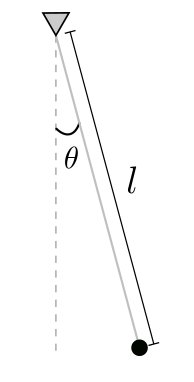
\includegraphics[scale=0.5]{figs/simplependulum.png}
    \caption{The Simple Pendulum}
    \label{simple}
\end{figure}

If a pendulum is set in motion so that is swings back and forth, its motion will be periodic. The time that it takes to make one complete oscillation is defined as the \textbf{time period} $T$ of the pendulum. Most of you will probably recognise the following formula for $T$: 

\begin{equation}
    T = 2 \pi \sqrt{\frac{l}{g}} 
    \label{TimeP}
\end{equation}

where $l$ is the length of the pendulum from its fixed point, and $g$ is the acceleration due to gravity. Not so many of you, however, will realise that this is only true for \textbf{small displacements} around the equilibrium position. In general, when the pendulum is displaced from its equilibrium position, it experiences a restoring force $m g \sin\theta$. The differential equation describing its motion can be obtained from Newton's Second Law  $m\vb{a} = \vb{F}$.

\begin{equation}
    m l \dv[2]{\theta}{t} = - m g \sin\theta
\end{equation}

This is a difficult differential equation to solve. In the approximation that the angle $\theta$ is very small, we can replace $\sin\theta \approx \theta$, and we are left with the following differential equation:

\begin{equation}
    \dv[2]{\theta}{t} + \frac{g}{l} \theta = 0
\end{equation}

It is in this approximation that the simple pendulum is a \textbf{simple harmonic oscillator}, a very important model that you will not stop seeing the end of. In general, a quantity $Q$ is considered observe simple harmonic variation with respect to some parameter $t$ (not necessarily time) if it satisfies the following differential equation:

\begin{equation*}
    \dv[2]{Q}{t} + \omega_0^2 Q = 0
\end{equation*}

where $\omega_0$ is the time period of the oscillation, and is related to the time period of the oscillation through 

\begin{equation*}
    T = \frac{2\pi}{\omega_0}
\end{equation*}

Comparing, you should see that in our case, $$\omega_0 = \sqrt{\frac{g}{l}}$$ and $$T = 2\pi \sqrt{\frac{l}{g}}$$

Thus, it should be clear that it is only when the amplitude is \textbf{small} that the time period follows this equation, since it is only then when you can approximate $\sin\theta$ with $\theta$.

In this introductory experiment you will begin by verifying the above formula for the time period for small angles. You will then attempt to explore any variation of the time period with angle.

\section{Apparatus}

\begin{enumerate}
    \item Metallic bobs of different materials
    \item A length of string
    \item A cork with a slit
    \item A retort stand with attached protractor
\end{enumerate}

\section{Suggested Procedure}

\paragraph{Question:} Which are the different physical quantities in this problem that can be varied to potentially change the time period\footnote{\textbf{Warning!} Do not use Equation (\ref{TimeP}) to answer this: we've already seen that that only works under certain special cases}?

\subsection{Part 1}

In this part of the experiment you will design a simple experiment to determine the variation of the time period with the mass of the bob.

\begin{enumerate}
    \item Begin by deciding which variables you need to fix, and which variables you will change.
    
    \item Draw out an appropriate table in your auxiliary notebooks. Mark out any important details that would help you remember what you've done when you re-read this. Remember to state not only what you have changed, but also what you have kept \textit{fixed}.
    
    \item Decide on the \textbf{number} of readings you will take. When you have arrived at a number, try to \textit{justify} it.
    
    \item Perform the necessary experiment, varying the relevant parameter. Note down your data.
    
    \item Plot an appropriate graph that accurately depicts your results.
\end{enumerate}

\paragraph{Question:} What is your conclusion? How confident are you of this conclusion?


\subsection{Part 2}

In this part of the experiment you will design a simple experiment to determine the variation of the time period with the length of the string from the pivot to the center of mass of the bob.

\begin{enumerate}
    \item Begin by deciding which variables you need to fix, and which variables you will change.
    
    \item Draw out an appropriate table in your auxiliary notebooks. Mark out any important details that would help you remember what you've done when you re-read this. Remember to state not only what you have changed, but also what you have kept \textit{fixed}.
    
    \item Decide on the \textbf{number} of readings you will take. When you have arrived at a number, try to \textit{justify} it.
    
    \item Perform the necessary experiment, varying the relevant parameter. Note down your data.
    
    \item Plot an appropriate graph that accurately depicts your results.
\end{enumerate}

\subsection{Part 3}

In this part of the experiment you will design a simple experiment to determine the variation of the time period with the angle of release of the bob.

\begin{enumerate}
    \item Begin by deciding which variables you need to fix, and which variables you will change.
    
    \item Draw out an appropriate table in your auxiliary notebooks. Mark out any important details that would help you remember what you've done when you re-read this. Remember to state not only what you have changed, but also what you have kept \textit{fixed}.
    
    \item Decide on the \textbf{number} of readings you will take. When you have arrived at a number, try to \textit{justify} it.
    
    \item Perform the necessary experiment, varying the relevant parameter. Note down your data.
    
    \item Plot an appropriate graph that accurately depicts your results.
\end{enumerate}


\paragraph{Note:} The repetition is -- of course -- intentional. We have found that students usually jump through these steps and -- as a result -- spend much of their time painstakingly collecting data that is of little or no use. It is essential that you spend some time deciding what exactly you want to collect, and how best you will represent it, before actually spending any time with the apparatus.



\section{Questions}

\paragraph{Question: } What would be the effect -- if any -- of changing the \textbf{shape} of the bob on the time period? Justify your answer.

\clearpage

\part{Experiments}
\title{Diffraction of Light}
\author{An Introduction to Physics through Experiments}
\date{}
\maketitle

\section*{Objectives}

\begin{enumerate}
    \item To determine the wavelength $\lambda$ of the light emitted by a laser source by studying the diffraction of light due to plane diffraction gratings.
    \item To determine the width of the given single slit by studying its diffraction pattern.
    \item To determine the diameter of a given wire by studying its diffraction pattern.
    \item To determine the size of the circular aperture by studying its diffraction pattern.
\end{enumerate}



\section*{Apparatus}

\begin{enumerate}
    \item A 10 mW seminconductor red laser source.
    \item A 5 mW DPSS green laser source.
    \item A set of necessary mounts.
    \item A set of plane diffraction gratings of different grating spacings.
    \item A single helix (spring) set in a holder
    \item A double helix set in a holder
    \item Measuring tapes.
    \item A holder for grating.
    \item A set of screens.  
    \item A single slit of fixed width mounted on a slide.
    \item Two multiple slits mounted on slides.
    \item Circular apertures mounted on slides.
    \item A spirit level
\end{enumerate}

\section*{Introduction}
	 
In Opticks (1704), Issac Newton wrote, ``Light is never known to follow crooked passages nor to bend into the shadow''. He explained this by describing how particles of light always travel in a straight line, and how objects kept in the path of the light cast a shadow because the particles can never spread out behind the object. However, a set of experiments on the propagation of light through small apertures performed by Francesco Grimaldi, Augustine Fresnel, Thomas Young and a few others firmly established that light actually enters into the shadow region with a definite pattern when it passes through around an edge. The resulting pattern depends on the relative size of the aperture or obstacle and the wavelength of light. If the size is much larger than the wavelength, the bending will be almost unnoticeable. However, if the two are similar in size, the diffraction will be considerable.    
     
In this experimental problem, we will use a low power solid-state laser as a source of an intense beam of monochromatic light. When light from a distant source (or a laser source) passes around a thin aperture or through a narrow aperture and is then intercepted by a viewing screen, the light produces a pattern on the screen called a \textit{diffraction pattern}. When such a beam is incident on various diffracting components like a plane diffraction grating, a single slit, a wire mesh or a two-dimensional diffraction grating, the light emerging from these components show a variety of interesting diffraction patterns. This pattern consists regions of maximum and minimum intensities, which characterise the diffracting object. 

\section*{Theory}

\subsection*{Plane Diffraction Grating}

A transmission diffraction grating consists of a large number of slits separated from one another by an opaque region. The grating concentrates the diffracted light along a particular direction in contrast to the single slit, which has a rather broad diffraction maximum. The maxima (bright intense spots) produced by a grating are usually called the principal maxima. They are quite intense and are also widely separated; what cannot be detected visually are the large number of secondary maxima which lie between neighboring principal maxima.

The expression, relating wavelength $\lambda$ of light used and the grating spacing $d$, with angle of deviation $\theta$ is,    
\begin{equation*}
    d \sin{\theta_m} = m \lambda,  \quad\quad\quad \text{for    m  = 1, 2, 3,}\hdots
\end{equation*}

In the above expression, $m$ represents the order of \textbf{maxima} points and the angle $\theta_m$  corresponds to  $m$th  order maximum intensity point. This relation is valid for a single slit and for the wire like obstacle.

Fig. 1

\subsection*{Single Slit}

When a (monochromatic) beam of light such as a laser is incident on a narrow single slit, the light emerging from the slit shows a diffraction pattern on a screen. The distribution of the intensity of light received on a screen show a pattern of varying intensity consisting of a bright central maximum with alternate minima and maxima of decreasing intensity on either side, known as a \textit{Fraunhofer diffraction pattern}.

The positions of the \textbf{minima} (zeros) of the intensity distribution pattern of a narrow slit due to a plane wave front (the Fraunhofer diffraction pattern) are given by the relation 

\begin{equation*}
    a \sin{\theta_m} = m \lambda  \quad\quad\quad \text{for    m  = 1, 2, 3,}\hdots,
\end{equation*}

where $\lambda$ is the wavelength of the incident light, $a$ is the width of the slit and $\theta_m$ is the angle corresponding to $m$th minimum. 

Fig. 2



\subsection*{Circular Aperture}

The diffraction pattern due to a circular aperture (known as an \textit{Airy diffraction pattern}) is similar to a single slit diffraction but the mathematics involved is more complicated which gives the expression nearly identical to that of the single slit. Hence we may apply the same expression to the diffraction due to a circular aperture, 

\begin{equation*}
    d \sin{\theta_m} = \overline{m} \lambda,  \quad\quad\quad \text{for    m  = 1, 2, 3,}\hdots
\end{equation*}

where $d$ is the diameter of the circular aperture and $\theta_m$ is the angle of deviation for the $m$th dark ring. The variable $\overline{m}$ has the following values:

\begin{equation*}
    \begin{aligned}
        m = 1 &\quad& \overline{m}=1.22
        m = 2 &\quad& \overline{m}=2.23
        m = 3 &\quad& \overline{m}=3.23
        m = 4 &\quad& \overline{m}=4.24
    \end{aligned}
\end{equation*}

\subsection*{Cylindrical wires}

 
 Fig. 3(a) Single cylindrical wire                                Fig. 3(b) Two wires

A laser beam of wavelength $\lambda$, falling normally on a cylindrical wire of diameter $a$ is diffracted in the direction perpendicular to the wire. The resulting intensity pattern as observed on a screen is shown in \ref{Fig. 3(a)}. It will not have escaped your attention that this pattern is very similar to that observed for a single slit. This is due to Babinet’s principle, which states that complementary objects produce the same diffraction pattern. The mathematics of this are far beyond the scope of this lab session.

The intensity distribution as a function of angle $\theta$ with the incident direction is given by

\begin{equation*}
    I(\theta) = I(0) \left( \frac{\sin \beta}{\beta} \right)^2, \quad \quad  \beta = \frac{\pi a \sin \theta}{\lambda}
\end{equation*}


The central spot ($\beta = 0$ and $\sin\beta = 0$) is bright. For other angles, when $\sin\beta=0$ but $\beta \neq 0$, the intensity vanishes.

Thus the intensity distribution has $n$th minimum at the angle $\theta_n$ given by

\begin{equation*}
    a \sin\theta_m = \pm m \lambda
\end{equation*}

Here the $\pm$ refers to either side of the central spot ($\theta = 0$).

The diffraction pattern due to two parallel identical wires of width $a$ kept at a distance $d$ from each other (Fig. 3(b)) is a combination of two patterns (diffraction due to a single wire and interference due to two wires).

The resultant intensity distribution is given by   

\begin{equation}
    I(\theta) = I(0) \cos^2\delta \left( \frac{\sin \beta}{\beta} \right)^2, \quad \quad  \beta = \frac{\pi a \sin \theta}{\lambda}, \delta = \frac{\pi d \sin \theta}{\lambda}
\end{equation}

For a screen placed at a large distance $D$ from the wire, the positions of the minima on the screen are observed at 

\begin{equation*}
    \begin{aligned}
        x_{\pm n} = \pm n \frac{\lambda D}{a}, &\quad& \text{due to diffraction},\\
        x_{\pm m} = \pm \left( m - \frac{1}{2}\right) \frac{\lambda D}{d}, &\quad& \text{due to interference}
    \end{aligned}
\end{equation*}


\subsection*{Single and double helices:}
  
               
Fig. 4 (a) A single helix Fig. 4 (b) A double helix

Now consider a set of four identical wires, the net intensity distribution is a combination of diffraction from each wire and interference due to pairs of wires and hence depends on $a$, $d$ and $s$ \ref{Figure 5 (a)}.

In other words, the combination of three different intensity patterns is observed.

  

Fig. 5 (a) Projection of a double helix    Fig. 5(b) Double helix given in the sample


\section*{Procedural Instructions}

\subsection*{Part A}

Observe effect of colour and also of white light on the diffraction pattern obtained by a suitable grating. Then choose an appropriate diffraction grating and perform the measurements to determine the wavelength $\lambda$ of the laser. 

\paragraph{Question:} Estimate the error in the value of the wavelength of light.

\paragraph{Question:} What are the sources of error in the above-determined value of $\lambda$ ? What measures should be taken to minimize these errors? 

Tilt the grating at an angle and see how this affects the diffraction pattern.

\subsection*{Part B}

Repeat Part A, for a different gratings (with different values of d), and calculate wavelength $\lambda$ as accurately as possible.

\subsection*{Part C}

Design and perform the necessary experiment with a single slit of fixed width and determine the width d of the given single slit.

Tilt the slit at an angle and see how this affects the diffraction pattern.

\subsection*{Part D}

Now take the given circular aperture as the diffracting object and determine the diameter of the circular aperture.

\subsection*{Part E}

Study of the diffraction pattern due to a helical spring and determine pitch of the spring and thickness of its wire. 

\paragraph{Question:} How does this part of the experiment relate to Part C? Can you explain the form of the diffraction pattern observed?

\subsection*{Part F}

Study of the diffraction pattern due to a double helix (as in our DNA) and determine all its parameters \ref{Fig 5 (b)}


\paragraph{Question} Explain how will be the diffraction pattern, observed using a laser source with
\begin{enumerate}[label=(\alph*)]
    \itemsep0em
    \item A fine wire mesh,
    \item A square aperture,
    \item A rectangular aperture.
\end{enumerate}




\subsection*{Precautions}

\begin{enumerate}
    \item Never look directly at a laser beam with the naked eye or any optical device. It may damage the eye permanently.
    \item Never allow a laser beam to shine in the area of anyone’s eye, as it is harmful to eyes.
    \item Never place highly reflective objects (such as rings, watches, and glassware) in the path of the laser beam.
    \item For proper working of laser, it should be kept ON throughout. Do not put it OFF until you complete all the readings, but if you do not need the laser beam for measurements or alignment, use the light-blocking screen to block the Laser beam.
    \item Treat the laser source as any other electrical device. It should never be tampered with, while the power cord is connected.
    
\end{enumerate}


\section*{References}

\begin{enumerate}
\itemsep0em
    \item Eric Stanley, Am. J. Phys., Vol.- 54, No.-10, October 1986, pp. 952.
    \item F.A. Jenkins, H.E. White, \textit{Fundamentals of Optics}, Third Edition, Mc-Graw Hill Kogakusha Ltd., Toyko, Japan, 1957, pp. 288-309, 328-350.
    \item F.W. Sears, \textit{Optics}, Third Edition, Asia Publishing House, 1958, pp 221-252.
    \item R.W. Ditchburn, \textit{Light}, Second Edition, The English Language Book Society and Blackie \& Son Ltd., 1963, pp 162-237.
    \item John Beynon, \textit{Introductory University Optics}, Prentice-Hall of India Pvt. Ltd., New Delhi (India), 1998, pp 158-190.
    \item Rajpal S. Sirohi, \textit{Wave Optics and its Applications}, Orient Longman Limited, (India), 1993, pp 169-210.
\end{enumerate}


\title{The Soft Massive Spring}
\author{An Introduction to Physics through Experiments}
\date{}

\maketitle

\section*{Objectives}

\begin{enumerate}
\item To determine the spring constant and the mass correction factor for the given soft massive
spring by static (equilibrium extension) method.
\item To determine the spring constant and the mass correction factor for the given soft massive
spring by dynamic (spring mass oscillations) method.
\item To determine the frequency of oscillations of the spring with one end fixed and the other
end free i.e. zero mass attached.
\item To study the longitudinal stationary waves and to determine the fundamental frequency of
oscillations of the spring with both the ends fixed.
\end{enumerate}

\section*{Apparatus}

\begin{enumerate}[label=\arabic*)]
\itemsep0em
\item A set of soft massive springs
\item A long and heavy retort stand with a clamp at the top end 
\item A set of masses with hooks
\item A signal generator (\textit{Equip-tronics QT-210})
\item A dual output power amplifier with the connecting cords
\item A mechanical vibrator
\item A digital multimeter (\textit{Victor VC97})
\item A digital stopwatch (\textit{Racer})
\item Measuring tapes
\item A set of measuring scales (1.0 m, 0.6 m and 0.3 m)
\end{enumerate}

\section*{Introduction}

A spring is a flexible elastic device which stores potential energy by the straining of the bonds between the atoms of the elastic material of which it is made. A variety of springs are available which are designed and fabricated to suit the various mechanical systems. Some common types of springs are compression springs, extension springs and torsion springs. 

Robert Hooke, a 17th century physicist, studied the behavior of springs under different loads. He established an equation, now known as Hooke’s law of elasticity which states that the amount by which a material body is deformed (the \textit{strain}) is linearly proportional to the force causing the deformation (the \textit{stress}). When applied to a spring, Hooke’s law implies that the restoring force is linearly proportional to the equilibrium extension. In other words,  $$F = - k x,$$ where $F$ is the restoring force exerted by the spring, $x$ is the displacement from the equilibrium position and $k$ is called the spring constant\footnote{The negative sign indicates that the force $F$ is opposite in direction to the extension $x$, hence the term `restoring'.}. For this equation to be valid, $x$ needs to be below the elastic limit of the spring. If $x$ is more than the elastic limit, the spring will exhibit `plastic behavior', where the atomic bonds in the material of the spring get broken or rearranged and the spring no longer returns to its original state. It may be noted that the potential energy $U$ stored in a spring is given by $$U= \frac{1}{2} k x^2$$

Depending on the value of the spring constant, a spring can be called \textit{soft} or \textit{hard}. A spring may also be considered to be massless or massive, depending on the mass that needs to be attached to it to get a considerable extension in the spring. Sometimes springs are also categorized by the ratio of spring constant to the mass of the spring $(\nicefrac{K}{m_s})$. A soft massive spring has a low spring constant and its mass can not be neglected. 

Ideal springs are considered to be massless. Hung vertically without any mass attached, an ideal spring shows no extension. Similarly, with an attached mass $M$ the spring is found to oscillate with a characteristic time period $$T = 2\pi \sqrt{\frac{M}{k}}$$ Practically (for example in the determination of its spring constant), we usually neglect the mass of the spring. However, if the spring extends under its own weight, its mass cannot be neglected and therefore the extension requires a correction. Similarly, they oscillate without any attached mass, implying that the standard formula for the time period of oscillations of a spring needs modification. The corrected formulae have been worked out and, interestingly, one finds that the correction factors $m_\text{corr}$ due to the spring's mass $m_s$ in these two cases are not the same. In this problem, we will experimentally study and verify the modified formulae. 

An extended soft massive spring clamped at both the ends can be assumed to be a uniformly distributed mass system. It has its own natural frequencies of oscillations (corresponding to different normal modes) like a hollow pipe closed at both the ends. Using the method of resonance we will excite and study different normal modes of vibrations of the spring. Here the longitudinal stationary waves will be set up on the extended soft massive spring. 

\section*{Description}

In \textbf{Part A}, we will use the static method, where the equilibrium extension of a given spring will be measured for different attached masses and the spring constant and the mass correction factor will be determined. 

In \textbf{Part B}, we will use the dynamic method, where different masses will be attached to the lower end of the spring with its upper end fixed and corresponding time period of oscillations for such a spring-mass system will be measured. The frequency of oscillations of the spring with the upper end fixed and the lower end free (i.e. with no attached mass) will be determined graphically. 

In \textbf{Part C}, we will use a mechanical vibrator to force oscillations on the spring and excite different normal modes of vibrations of the spring. Thus the longitudinal stationary waves will be set up on the spring. We will measure the frequencies of the excitations corresponding to different normal modes. From these, the fundamental frequency of oscillation with both the ends fixed will be determined. We will compare this frequency with the frequency of oscillations with one end fixed and the other end free as determined earlier in Part B.



\section*{Theory}

\subsection*{Part A}

Let $L_0$ be the length of the spring when the spring is kept horizontal under no tension, $m$ be
the mass attached to the free end of the spring, $L_m$ be the length of the spring when the mass
is attached at its lower end, $S_m$ be the equilibrium extension of the spring for mass $m$, $m_s$ be the mass of the spring, $k$ be the spring constant and $g$ be the acceleration due to gravity.

Thus,

\begin{equation}
S_m = L_m - L_0
\end{equation}

We can determine the expression for $S_m$, by taking extension of a small element and integrating over the total length of the spring,

\begin{equation}
S_m = \left( m + \frac{m_s}{2} \right)\left(\frac{g}{k} \right)
\end{equation}

The factor $(\nicefrac{m_s}{2})$ is known as the mass correction factor in the \textbf{static} case.


\subsection*{Part B}
In case of the soft massive springs, we cannot neglect the mass of the spring since these springs can oscillate without any attached mass. We thus need to modify the earlier expression for $T$. This can be done using the principle of conservation of energy, $$\text{Potential Energy + Kinetic Energy = constant.}$$

The modified expression is found to be

\begin{equation}
T = 2\pi \sqrt{\cfrac{\left(m + \cfrac{m_s}{3}\right)}{k}}
\end{equation}

The factor $(\nicefrac{m_s}{3})$ is known as the mass correction factor in the \textbf{dynamic} case. Note that this factor is different from the mass correction factor in the previous (static) case.

The corresponding frequency is given by $$f_0 = \frac{1}{T}$$


\subsection*{Part C}

As mentioned earlier, the extended spring has its own natural frequencies like a hollow pipe closed at both the ends. Note that both the ends of the spring may be taken to be fixed in the case in question: the upper end is fixed in any case and the amplitude of the lower end is small, as compared to the extended length of the spring, and can be taken to be nearly zero. The natural frequencies correspond to stationary waves; their wavelengths are given by 

\begin{equation*}
\lambda_n = \left( \frac{2}{n}\right) L , \quad \quad n=1,2,3\hdots
\end{equation*}

We know that the speed $v$ of the waves on the spring follow the equation $$v = f_n \lambda_n$$ Thus,

\begin{equation}
\begin{aligned}
f_n = \frac{v}{\lambda_n} &= \frac{v n}{2L}\\
f_1 = \frac{v}{2L}, \quad f_2 = \frac{v}{L},\quad &\hdots,\quad f_n = n f_1
\end{aligned}
\end{equation}

\section*{Experimental Setup}

For Parts A and B, you will need a soft massive spring, a retort stand with a clamp, a set of
masses, a measuring tape or scales and a digital stopwatch. For Part C, you will need a soft massive spring, a long and heavy retort stand with a clamp at the top and a mechanical vibrator clamped near the base of the stand. We will also need a function generator. In this case, the soft massive spring should be clamped at the upper end of the stand. The lower end of the spring should be clamped to the crocodile clip fixed at the centre of the mechanical vibrator. The lower end of the spring will be subjected to an up and down harmonic motion using the mechanical vibrator. It must be ensured that the amplitude of this motion is small enough so that these ends could be considered to be fixed.

\subsection*{Warnings}

\begin{itemize}
\item Do not extend the spring beyond the elastic limit. Choose the value of the maximum mass that may be attached to the lower end of the given spring carefully.
\item Keep the amplitude of oscillations of the spring-mass system just sufficient to get the required number of oscillations.
\item The amplitude of vibrations should be carefully adjusted to the required level using the amplitude knob of the function generator so as to not blow the fuse in the power amplifier. The brighter and more frequently the indicator LEDs flash indicates that the fuse is close to blowing.
\end{itemize}

\section*{Procedural Instructions}

\subsection*{Part A}
\begin{enumerate}
\item Measure the length $L_0$ of the spring keeping it horizontal on a table in an unstretched (all the coils touching each other) position.
\item Hang the spring to the clamp fixed to the top end of the retort stand. The spring extends under its own weight.
\item Take appropriate masses and attach them to the lower end of the spring. 
\item Measure the length $L_m$ of the spring in each case. (For better results you may repeat
each measurement two or three times.) Thus determine the equilibrium extension $S_m$ for each value of mass attached.
\item Plot an appropriate graph and determine the spring constant $k$ of the spring and the mass of the spring $m_s$.
\end{enumerate}

\paragraph{Question 1:} State and justify the selection of variables plotted on the $x$ and $y$ axes. Explain the observed behavior and interpret the $x$ and $y$ intercepts.



\subsection*{Part B}

\begin{enumerate}
\item Keep the spring clamped to the retort stand.

\item Try to set the spring into oscillations without any mass attached, you will observe that
the spring oscillates under the influence of its own weight.

\item Attach different masses to the lower end of the spring and measure the time period of oscillations of the spring mass system for each value of the mass attached. You may measure the time for a number of oscillations to determine the average time period.

\item Perform the necessary data analysis and determine spring constant $k$ and the mass of the spring $m_s$ using the above data. Compare these values to those obtained in the Part A.

\item Also determine frequency $f_0$ for zero mass attached to the spring from the graph.


\paragraph{Question 2:} Does the above method of measuring the total time for a number of oscillations help us to increase the reliability of time period measurement?
\end{enumerate}


\subsection*{Part C}

\begin{enumerate}
\item Keep the spring clamped to the long retort stand.

\item Clamp the lower end of the spring to the crocodile clip attached to the vibrator.

\item Connect the output of the function generator to the input of the mechanical vibrator
through the power amplifier, using the BNC cable.

\item Starting from zero, slowly go on increasing the frequency of vibrations produced by the vibrator by increasing the frequency of the sinusoidal signal generated by the function generator. At one particular frequency you will observe that the midpoint of the spring oscillate with large amplitude indicating an antinode. (You may use a small piece of tissue paper to observe the amplitude at the antinode.) This is the fundamental mode (first harmonic) of oscillation of the spring. Adjust the frequency to get the maximum possible amplitude at the antinode. Measure and record this frequency using the frequency setting on the multimeter.

\item You will find, however, that it is easier to locate nodes (places where the spring does not move) than antinodes. Increase the frequency further and observe higher harmonics identifying them on the basis of the number of loops you can see between the fixed ends. (If you see $n$ nodes -- or fixed points -- between the endpoints, there are $n+1$ loops.)

\item Plot a graph of frequency for different number of loops versus the number of loops. Determine this fundamental frequency $f_1$ from the slope of this graph.

\item Compare this fundamental frequency $f_1$ with the frequency $f_0$ of the spring mass
system with one end fixed and the zero mass attached (as determined in Part B) and
show that $$f_0 = \nicefrac{f_1}{2}$$
\end{enumerate}

\paragraph{Question 3:} Explain why the two frequencies should be related by a factor of two? (You may use the analogy between the spring and an air column.)


\section*{References}

\begin{enumerate}
\itemsep0em
\item J. Christensen, \textit{Am. J. Phys}, 2004, 72(6), 818-828.

\item T. C. Heard, N. D. Newby Jr, Behavior of a Soft Spring, \textit{Am. J. Phys}, 45 (11), 1977,
pp. 1102-1106. 

\item H. C. Pradhan, B. N. Meera, Oscillations of a Spring With Non-negligible Mass, \textit{Physics Education (India)}, 13, 1996, pp. 189-193.

\item B. N. Meera, H. C. Pradhan, Experimental Study of Oscillations of a Spring with Mass Correction, \textit{Physics Education (India)}, 13, 1996, pp. 248-255.

\item Rajesh B. Khaparde, B. N. Meera, H. C. Pradhan, Study of Stationary Longitudinal Oscillations on a Soft Spring, \textit{Physics Education (India)}, 14, 1997, pp. 130-19. 

\item H. J. Pain, \textit{The Physics of Vibrations and Waves}, 2nd Ed, John Wiley \& Sons, Ltd., 1981.

\item D. Halliday, R. Resnick, J. Walker, \textit{Fundamentals of Physics}, 5th Ed, John Wiley \& Sons, Inc., 1997.

\item K. Rama Reddy, S. B. Badami, V. Balasubramanian, \textit{Oscillations and Waves}, University
Press, Hyderabad, 1994.
\end{enumerate}


\clearpage
\pagenumbering{arabic} 

\title{The Three-Terminal Black Box}
\author{An Introduction to Physics through Experiments}
\date{}

\maketitle

\section*{Objectives}

\begin{enumerate}
\item To study a three-terminal black box and identify the circuit within it along with the values of the electronic components.

\item To understand the responses of different active and passive circuit elements and their combinations, and learn to recognise them.

\item To exercise your deductive and inductive powers, much as real physicists must do with real experiments.

\end{enumerate}




\section*{Apparatus}

\begin{enumerate}
\item A black box with three connecting terminals marked A, B and C
\item A variable DC power supply (\textit{Keltronix})
\item Two digital multimeters (\textit{MECO 603})
\item A signal generator (\textit{Testronix 72})
\item A Digital Storage Oscilloscope (\textit{GW INSTEK–GDS-1102U})
\item A digital stopwatch (\textit{Racer})
\item A resistor ladder
\item Connecting wires

\end{enumerate}


\section*{Introduction}

You are given a sealed box on which three terminals marked A, B and C are provided which connect to a circuit inside. The circuit inside the box consists of \textbf{three} electronic components of different kinds (i.e. resistors, p-n junction diodes, batteries, etc.). Please note that the black box may consist of combinations of either only one or only two or three types of components. 

The components may be connected in either a `star' or `delta' connection (refer to the theory section for details). You are expected to identify the interior components as to type and value, and determine how they are connected to each other and to the terminals. 


\section*{Description}

In \textbf{Part A}, the black box will contain only combinations of resistors, p-n junction diodes, and batteries in a \textit{star} connection.

In \textbf{Part B} \textit{(optional)}, the black box will contain only combinations of resistors, p-n junction diodes and capacitors in a \textit{star} connection. 

In \textbf{Part C} \textit{(optional)}, the black box will contain only combinations of resistors, p-n junction diodes, and batteries in a \textit{delta} connection. 

In \textbf{Part D} \textit{(optional)}, the black box will contain only combinations of  resistors, capacitors, and inductors in a \textit{star} connection.


\section*{Theory}

\subsection*{Star and Delta Connections}

Standard 3-component circuits take on two major forms with names that represent the way in which the components are connected: a \textbf{Star} sometimes represented by Y, and a Delta connected network sometimes represented by a triangle or $\Delta$. Both these forms, represented in Figure (\ref{starAndDelta}), are indistinguishable from each other, in that for every star connection there is an equivalent delta connection (with different values for the individual components) and vice versa. It is for this reason that you must keep in mind what form the black box is in before drawing any conclusions.

\begin{figure}[!htb]
       \begin{subfigure}[t]{0.3\textwidth}
				\centering
                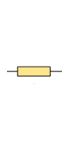
\includegraphics[scale=0.8]{comp.png}
                \captionsetup{justification=centering}
                \caption{Component or combination \\of components}
       \end{subfigure}%
       \begin{subfigure}[t]{0.3\textwidth}
				\centering
                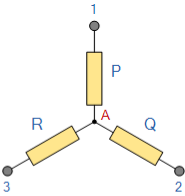
\includegraphics[scale=0.6]{star.png}
                \caption{Star connection}
        \end{subfigure}%
        \begin{subfigure}[t]{0.3\textwidth}
        		\centering
                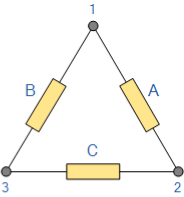
\includegraphics[scale=0.6]{delta.png}
                \caption{Delta connection}
        \end{subfigure}%
        \caption{Circuit connections}
        \label{starAndDelta}
\end{figure}

\begin{figure}[!htb]
\centering
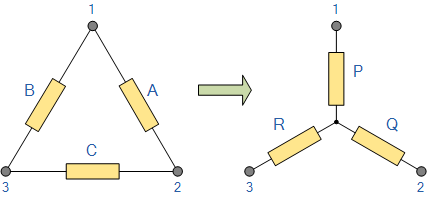
\includegraphics[scale=0.6]{stardelta.png}
\caption{Star to Delta conversion}
\label{starToDelta}
\end{figure}

The following formulae will allow you to move between a star connection and its associated delta connection and vice versa:

\begin{minipage}{0.5\textwidth}
\centering
\paragraph*{Delta to Star Network:}
\begin{equation*}
\begin{aligned}
P &= \frac{A B}{A + B + C}\\
Q &= \frac{A C}{A + B + C}\\
P &= \frac{B C}{A + B + C}\\
\end{aligned}
\end{equation*}
\end{minipage}
\begin{minipage}{0.5\textwidth}
\centering
\paragraph*{Star to Delta Network:}
\begin{equation*}
\begin{aligned}
A &= \frac{P Q + Q R + R P}{R}\\
B &= \frac{P Q + Q R + R P}{Q}\\
C &= \frac{P Q + Q R + R P}{P}\\
\end{aligned}
\end{equation*}

\end{minipage}


\subsection*{Passive circuit components}

Passive circuit components are electrical components that cannot control the current in a circuit. They do not generate power, but instead dissipate, store, and/or release it. Some such components are discussed below.

\subsubsection*{Resistors}

A resistor is a two-terminal passive electronics component used to oppose or limit the current in a circuit. A resistor works based on the principle of Ohm’s law which states that the voltage applied across the terminals of a resistor is directly proportional to the current flowing through it, with the constant of proportionality called the \textit{resistance}.

\begin{equation*}
V = I R
\end{equation*}

\subsubsection*{Capacitors}

A capacitor, made from two conductive plates with an insulator between them, stores electrical energy in the form of an electric field. It blocks the DC signals and allows the AC signals to pass through it. The charge stored in a capacitor is given by

\begin{equation*}
Q = CV
\end{equation*}

When used with a resistor, the time a capacitor takes to charge or discharge is measured in units of an intrinsic time scale, known as the time constant $\tau = RC$ of the circuit.

\subsection*{Active circuit components}
An active device is any type of circuit component with the ability to electrically control electron flow in the circuit.

\subsubsection*{Batteries}

Charges can be separated by several means to produce a voltage. A battery uses a chemical reaction to produce energy and separate opposite sign charges onto its two terminals. As the charge is drawn off by an external circuit, doing work and finally returning to the opposite terminal, more chemicals in the battery react to restore the charge difference and the voltage.


\subsubsection*{p-n junction Diodes}

A p-n junction diode is two-terminal semiconductor device, which allows the electric current in only one direction while blocks the electric current in opposite or reverse direction. Such a diode has an anode (or positive end) containing positive charge carriers called `holes', and a cathode (or negative end) containing negative charge carriers or electrons. The interface between these ends forms a region without any charge carriers called the \textbf{depletion layer}. 

The process of applying the external voltage to a p-n junction semiconductor diode is called biasing. If the diode is \textbf{forward biased} -- that is, when a positive voltage is applied to the anode and a negative voltage to the cathode -- it allows the charge carriers, and hence electric current, to flow. On the other hand, if the diode is \textbf{reverse biased} -- negative to the anode and positive to the cathode -- it blocks the current flow. In the conventional symbol for a diode, the arrowhead indicates the conventional direction of electric current when the diode is forward biased.

Unlike a resistor, a diode does not behave linearly with respect to the applied voltage as the diode has an exponential current-voltage (I-V) relationship and therefore cannot be described by simply using an equation such as Ohm’s law. The basic reason for this is that the width of the depletion layer decreases with increase in positive voltage. After a certain `knee' voltage (0.3 V for Germanium semiconductors and 0.7V for Silicon semiconductors) the width of the barrier effectively goes to zero, and the diode acts like a short circuit with zero resistance. When a junction diode is reverse biased the thickness of the depletion region increases and the diode acts like an open circuit blocking any current flow (except only a very small leakage current), until an `avalanche' voltage when the device overheats and gets shorted leading again to maximum current flow in the opposite direction.

\begin{figure}[!htb]
\centering
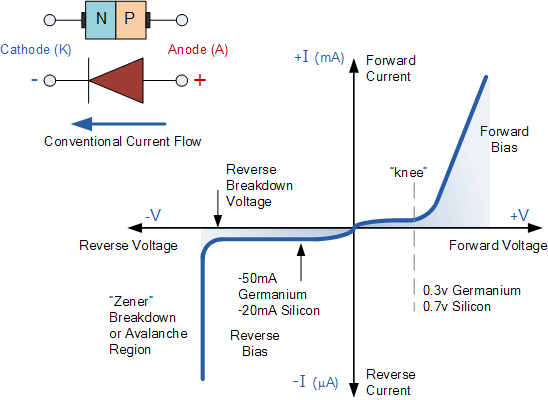
\includegraphics[scale=0.6]{diodeChar.png}
\caption{Diodes and their characteristics}
\label{diodeChar}
\end{figure}



\section*{Experimental Setup}


\subsection*{Black Box}
The black box contains an unknown circuit inside it which is connected to terminals A, B, and C in either a `star' or a `delta' connection (explained above). You have to use these for your analysis and measurements. Do not try to open the given black box.

\subsection*{Digital Multimeter (\textit{MECO 603})}

A multimeter is an instrument used to measure multiple parameters like voltage, current, and resistance. In this experiment you will use the given digital multimeters (Model \textit{MECO - 603}) \textbf{\textit{only}} for the measurement of DC and AC voltage and current. You will have to use input sockets marked COM, V/$\Omega$ and mA (or 20A) for the required measurements. Note that there are two input sockets marked mA and 20A for the current measurement. The socket marked mA may be used for measuring current below 250 mA and socket marked 20A may be used for measuring current up to 20 A. You will have to select the appropriate function and the range using the rotary switch provided on the multimeter. The value of voltage or current is displayed on the LCD screen. The multimeter is turned off by turning the dial to the appropriate setting.

\subsection*{Variable DC Power Supply (\textit{Keltronix})}

The power switch can be used to switch it ON or OFF. The required output can be taken from the two output terminals. The voltage and the current capacity can be changed using the three knobs: voltage coarse, voltage fine, and current. The given power supply also displays the value sof the output voltage and current. Do not use these value since measuring these values using given calibrated multimeter will be more reliable. 

The DC Variable Power Supply can either act as a source of Constant Current (CC) or Constant Voltage (CV), indicated by the two LEDs present on it. In general, most types of circuits require a constant voltage to operate, so if the CV LED is lit, the supply is working fine with your circuit. The power supply has a physical limit on how much current it can supply, if the load (your circuit) attempts to draw more, the power supply decreases the output voltage to keep the current consumed at its maximum permissible amount. For this experiment, you should turn the current dial up to the maximum. This allows the supply to work as a constant voltage supply unless the current drawn by your circuit goes beyond 1A.

\subsection*{Function Generator (\textit{Testronix 72})}

A function generator is a type of signal generator that is used to generate simple repetitive waveforms in the form of an alternating electrical wave. Typically, it will produce waveforms or functions such as sine waves, sawtooth waveforms, square, and triangular waveforms, and will allow you to adjust the frequency and amplitude of  the signals. The instrument given to you generates sine and square waveforms. The output may be taken from the output sockets for the respective waveforms. The frequency can be adjusted by turning the dial and selecting the appropriate Frequency Multiplier button. For example, turning the dial to 3 and selecting the 10k button would provide an output waveform with a frequency of 30kHz. Similarly the amplitude switch, used in conjunction with the appropriate buttons, can be used to adjust the amplitude of the output waveform from under 0V to 30V.



\subsection*{Warnings}

\begin{enumerate}
\item The use of a multimeter to measure the resistance is strictly prohibited.
\item Do not try to open the black box, use only terminals A, B and C for the connections.
\item Use fixed value resistors to prevent large currents in the circuit. The current should not exceed 50 mA.
\item \textbf{Do not} short the outputs of the power supply, it could damage the equipment.
\item Passing more current through the multimeter's (250 mA or 20A) sockets than they can handle will cause the fuses in the multimeter to burn out, leading to an open circuit. Use an appropriate resistance to limit the current in the circuit.
\item When drawing circuit diagrams use the standard symbols.
\item The digital multimeter, the DC power supply or the signal generator should be turned off if not in use.

\end{enumerate}


\section*{Procedural Instructions}

Design the most appropriate method to identify the circuit and determine the values of the electronic components used  in it. Give your answer in the form of a circuit diagram showing the terminals A, B, and C clearly. You will need to give \textit{all} the information required in order to reconstruct the circuit. For example, if you are doing Part A, you will need to determine the values of the resistors, the orientation of the diodes, and the voltage and orientation of the battery, if any of the above are used in the circuit.

In every part, clearly report the procedural steps you have taken with reference to your complete plan of experiment, the data will you collect, how the collected data will be analysed and finally the interpretation of your analysis. Your reporting should be comprehensive, and you are expected to mention all important procedural steps in your answer sheet.



\section*{References}

\begin{enumerate}

\item \href{https://www.elprocus.com/major-electronic-components/}{Overview of Various Basic Electronics Components}

\item \href{https://www.electronics-tutorials.ws/dccircuits/dcp_10.html}{Star Delta Transformation}

\item \href{https://www.electronics-tutorials.ws/diode/diode_3.html}{Electronics Tutorials: PN Junction Diode}

\end{enumerate}



\clearpage
\pagenumbering{arabic} 
 
\title{The Incandescent Lamp and the Inverse Square Law}
\author{An Introduction to Physics through Experiments}
\date{}

\maketitle

\section*{Objectives}

\begin{enumerate}
\item To understand the current-voltage characteristics of an incandescent lamp's filament.
\item To understand the dependence of the lamp's power on the resistance of its filament.
\item To observe and understand the variation of intensity with distance for a point source.
\end{enumerate}




\section*{Apparatus}

\begin{enumerate}
\item A DC variable power supply (\textit{Optochem})
\item Two digital multimeters with probes (\textit{MECO 603} and \textit{Victor VC97})
\item A 12 V, 21W incandescent lamp
\item A stand to hold the lamp
\item A Resistor Ladder
\item Connecting cords
\item A convex lens
\item A photodiode

\end{enumerate}


\section*{Introduction}



\section*{Description}

In \textbf{Part A}, you will design an experiment to study the VI characteristics of an incandescent lamp. 

In \textbf{Part B}, you will design an experiment to observe the variation of the lamp's power with the resistance of its filament. 

In \textbf{Part C}, you will design an experiment to create a point source and then observe the variation of its intensity as a function of the distance from the source. 


\section*{Theory}

\subsection*{Part A}

If an electric current is passed through a wire of significant resistance, the wire will be heated. If the wire is heated to a sufficiently high temperature, it will give off light.  This is the basis of a resistive incandescent lamp. The high melting point of tungsten (3680 K) and its low vaporization pressure makes it a suitable material to be used as the filament of almost all incandescent lamps. The brightness and the overall colour of emitted light depends on the temperature of the filament for a given lamp, which is a non-linear resistive element.

It is observed that (for a specific range of current) almost all incandescent lamps satisfy the relation

\begin{equation*}
V = K I^a
\end{equation*}

where $V$ is the voltage across the lamp, $I$ the current passing through the lamp, and $K$ and $a$ are constants.

\subsection*{Part B}


One finds for the resistive lamp, the empirical relation

\begin{equation*}
P = C R^n
\end{equation*}

where $P$ is the power supplied to the lamp, $R$ is the resistance of the filament of the lamp, and $n$ and $C$ are constants whose values depend on the material used for the filament of the lamp. The above relation yields better results when the temperature of the filament of the lamp is approximately above 1800 K for the given lamp. For such temperatures the resistance R of the lamp is found to be directly proportional to the absolute temperature T of the filament of the lamp.



\subsection*{Part C}


\begin{minipage}{0.5\linewidth}
%\vspace{-1.5cm}
A \textbf{point source} is a single identifiable localised source of, say, light. Such a source has negligible extent, distinguishing it from other source geometries, and are called point sources because in mathematical modeling, they can usually be approximated as a mathematical point to simplify analysis. The actual source need not be physically small, if its size is negligible relative to other length scales in the problem. For example, in astronomy, stars are routinely treated as point sources, even though they are in actuality much larger than the Earth.

For light or sound waves, a point source radiates the same intensity of radiation in all directions. That is, it has no preferred direction of radiation and radiates uniformly in all directions over a sphere centred on the source.
\end{minipage}
\begin{minipage}{0.5\linewidth}
\centering
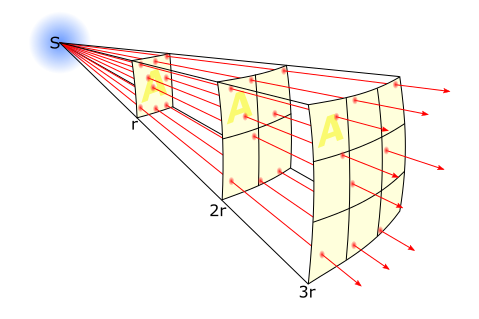
\includegraphics[scale=0.7]{isl.png}
\end{minipage}



\section*{Experimental Setup}

\subsection*{Digital Multimeter (\textit{MECO 603})}

A multimeter is an instrument used to measure multiple parameters like voltage, current, and resistance. In this experiment you are given two digital multimeters (Models \textit{MECO - 603} and \textit{Victor VC97})\footnote{The Victor multimeter has a greater current sensitivity.}. You will have to use input sockets marked COM, V/$\Omega$ and mA (or A or 20A) for the required measurements. Note that there are two input sockets marked mA and 20A (10A for the Victor multimeter) for the current measurement. The socket marked mA may be used for measuring current below 250 mA and socket marked 20A (or 10A) may be used for measuring current up to 20 A (or 10A). You will have to select the appropriate function and the range using the rotary switch provided on the multimeter. The value of voltage or current is displayed on the LCD screen. The multimeter is turned off by turning the dial to the appropriate setting.

\subsection*{Variable DC Power Supply (\textit{Optochem})}

The power switch can be used to switch it ON or OFF. The required output can be taken from the two output terminals. The voltage and the current capacity can be changed using the three knobs: voltage coarse, voltage fine, and current. The given power supply also displays the values of the output voltage and current. Do not use these value since measuring these values using given calibrated multimeter will be more reliable. 

The DC Variable Power Supply can either act as a source of Constant Current (CC) or Constant Voltage (CV). In general, most types of circuits require a constant voltage to operate. The power supply has a physical limit on how much current it can supply, if the load (your circuit) attempts to draw more, the power supply decreases the output voltage to keep the current consumed at its maximum permissible amount. For this experiment, you should turn the current dial up to the maximum. This allows the supply to work as a constant voltage supply unless the current drawn by your circuit goes beyond 2A.

\subsection*{Photodiode}

A photodiode is a semiconductor device that converts light into an electrical current. The current is generated when photons of sufficient energy are absorbed in the photodiode, creating an electron-hole pair through the photoelectric effect.

\subsection*{Warnings}

\begin{enumerate}
\item Do not apply a voltage more than 12 V to the lamp.
\item Clamp the lamp carefully on the retort stand so that it should not be damaged or the wires should not get shorted.
\item You will have to use the given fixed value resistor to control the current in the circuit.
\item Use the digital multimeter for the measurement of D.C. voltage and current.  Choose the most appropriate range for the measurement.
\item The incandescent lamp should not be kept connected to the power supply for long duration. 

\item Passing more current through the multimeter's (250 mA or 20A) sockets than they can handle will cause the fuses in the multimeter to burn out, leading to an open circuit. Use an appropriate resistance to limit the current in the circuit.

\item When drawing circuit diagrams use the standard symbols.

\item The digital multimeter, the DC power supply or the signal generator should be turned off if not in use.

\end{enumerate}


\section*{Procedural Instructions}

\subsection*{Part A}

You have to design and perform an experiment to determine the value of constant a for the given incandescent lamp, given that it follows the equation 

\begin{equation*}
V = K I^a
\end{equation*}

You will have to plot an appropriate graph and from the graph determine the value of $a$. Draw the necessary circuit diagram in your answer sheet.

\paragraph{Question:} How does the resistance of the lamp vary with the current?  Explain the cause of variation of the resistance of the lamp with the current?

\subsection*{Part B}

You have to design an appropriate procedure to determine the value of $n$. You may use the data gathered earlier, or you may perform new measurements. Plot the appropriate graph to determine the value of $n$.

\subsection*{Part C}

In this part, you have to study the fall of intensity of light emitted by the given incandescent lamp.  For this you have to use the given photodiode with a digital multimeter to measure the intensity of light. We assume that the relation between the intensity of light incident on the sensing area of the photodiode and its output current is linear. 

Use the converging lens that we have provided you with in order to create a point source. You may use the screen with a hole in it to allow the passage of a small amount of light of this `point source' that may then be detected by the photodiode. This screen will now act as your source.

Connect the output of the power supply to the given lamp and adjust the voltage applied to the lamp to be around 12 V. Keep the photodiode initially as close as possible to the screen acting as your source.  Study the variation of current IPD in the photodiode with the distance $d$ between the source and the photodiode. (You have to take readings for the value of $d$ varying from around 7.0 cm to around 50.0 cm.) You may have to correct your readings to account for the ambient light falling on the photodiode. 

Plot an appropriate linear graph to show the variation of the intensity of light with distance $d$.

\paragraph{Question:} What type of graph would be the most efficient to determine the variation of the intensity of light with distance?

\paragraph{Question:} After plotting this graph, you may find that points below 20.0 cm do not behave as you would expect them to. Can you explain why this is the case?


\section*{References}

\begin{enumerate}

\item \href{https://www.fh-muenster.de/ciw/downloads/personal/juestel/juestel/4-InkohaerenteLichtquellen-Glueh-_und_Halogenlampen_english_-1.pdf}{Incandescent and Halogen Lamps}

\item \href{https://www.elprocus.com/photodiode-working-principle-applications/}{Photodiode Working Principle, Characteristics and Applications}

\end{enumerate}

\clearpage
\pagenumbering{arabic} 

\title{Diffraction of Light}
\author{An Introduction to Physics through Experiments}
\date{}
\maketitle

\section*{Objectives}

\begin{enumerate}
    \item To determine the wavelength $\lambda$ of the light emitted by a laser source by studying the diffraction of light due to plane diffraction gratings.
    \item To determine the width of the given single slit by studying its diffraction pattern.
    \item To determine the diameter of a given wire by studying its diffraction pattern.
    \item To determine the size of the circular aperture by studying its diffraction pattern.
\end{enumerate}



\section*{Apparatus}

\begin{enumerate}
    \item A 10 mW seminconductor red laser source.
    \item A 5 mW DPSS green laser source.
    \item A set of necessary mounts.
    \item A set of plane diffraction gratings of different grating spacings.
    \item A single helix (spring) set in a holder
    \item A double helix set in a holder
    \item Measuring tapes.
    \item A holder for grating.
    \item A set of screens.  
    \item A single slit of fixed width mounted on a slide.
    \item Two multiple slits mounted on slides.
    \item Circular apertures mounted on slides.
    \item A spirit level
\end{enumerate}

\section*{Introduction}
	 
In Opticks (1704), Issac Newton wrote, ``Light is never known to follow crooked passages nor to bend into the shadow''. He explained this by describing how particles of light always travel in a straight line, and how objects kept in the path of the light cast a shadow because the particles can never spread out behind the object. However, a set of experiments on the propagation of light through small apertures performed by Francesco Grimaldi, Augustine Fresnel, Thomas Young and a few others firmly established that light actually enters into the shadow region with a definite pattern when it passes through around an edge. The resulting pattern depends on the relative size of the aperture or obstacle and the wavelength of light. If the size is much larger than the wavelength, the bending will be almost unnoticeable. However, if the two are similar in size, the diffraction will be considerable.    
     
In this experimental problem, we will use a low power solid-state laser as a source of an intense beam of monochromatic light. When light from a distant source (or a laser source) passes around a thin aperture or through a narrow aperture and is then intercepted by a viewing screen, the light produces a pattern on the screen called a \textit{diffraction pattern}. When such a beam is incident on various diffracting components like a plane diffraction grating, a single slit, a wire mesh or a two-dimensional diffraction grating, the light emerging from these components show a variety of interesting diffraction patterns. This pattern consists regions of maximum and minimum intensities, which characterise the diffracting object. 

\section*{Theory}

\subsection*{Plane Diffraction Grating}

A transmission diffraction grating consists of a large number of slits separated from one another by an opaque region. The grating concentrates the diffracted light along a particular direction in contrast to the single slit, which has a rather broad diffraction maximum. The maxima (bright intense spots) produced by a grating are usually called the principal maxima. They are quite intense and are also widely separated; what cannot be detected visually are the large number of secondary maxima which lie between neighboring principal maxima.

The expression, relating wavelength $\lambda$ of light used and the grating spacing $d$, with angle of deviation $\theta$ is,    
\begin{equation*}
    d \sin{\theta_m} = m \lambda,  \quad\quad\quad \text{for    m  = 1, 2, 3,}\hdots
\end{equation*}

In the above expression, $m$ represents the order of \textbf{maxima} points and the angle $\theta_m$  corresponds to  $m$th  order maximum intensity point. This relation is valid for a single slit and for the wire like obstacle.

Fig. 1

\subsection*{Single Slit}

When a (monochromatic) beam of light such as a laser is incident on a narrow single slit, the light emerging from the slit shows a diffraction pattern on a screen. The distribution of the intensity of light received on a screen show a pattern of varying intensity consisting of a bright central maximum with alternate minima and maxima of decreasing intensity on either side, known as a \textit{Fraunhofer diffraction pattern}.

The positions of the \textbf{minima} (zeros) of the intensity distribution pattern of a narrow slit due to a plane wave front (the Fraunhofer diffraction pattern) are given by the relation 

\begin{equation*}
    a \sin{\theta_m} = m \lambda  \quad\quad\quad \text{for    m  = 1, 2, 3,}\hdots,
\end{equation*}

where $\lambda$ is the wavelength of the incident light, $a$ is the width of the slit and $\theta_m$ is the angle corresponding to $m$th minimum. 

Fig. 2



\subsection*{Circular Aperture}

The diffraction pattern due to a circular aperture (known as an \textit{Airy diffraction pattern}) is similar to a single slit diffraction but the mathematics involved is more complicated which gives the expression nearly identical to that of the single slit. Hence we may apply the same expression to the diffraction due to a circular aperture, 

\begin{equation*}
    d \sin{\theta_m} = \overline{m} \lambda,  \quad\quad\quad \text{for    m  = 1, 2, 3,}\hdots
\end{equation*}

where $d$ is the diameter of the circular aperture and $\theta_m$ is the angle of deviation for the $m$th dark ring. The variable $\overline{m}$ has the following values:

\begin{equation*}
    \begin{aligned}
        m = 1 &\quad& \overline{m}=1.22
        m = 2 &\quad& \overline{m}=2.23
        m = 3 &\quad& \overline{m}=3.23
        m = 4 &\quad& \overline{m}=4.24
    \end{aligned}
\end{equation*}

\subsection*{Cylindrical wires}

 
 Fig. 3(a) Single cylindrical wire                                Fig. 3(b) Two wires

A laser beam of wavelength $\lambda$, falling normally on a cylindrical wire of diameter $a$ is diffracted in the direction perpendicular to the wire. The resulting intensity pattern as observed on a screen is shown in \ref{Fig. 3(a)}. It will not have escaped your attention that this pattern is very similar to that observed for a single slit. This is due to Babinet’s principle, which states that complementary objects produce the same diffraction pattern. The mathematics of this are far beyond the scope of this lab session.

The intensity distribution as a function of angle $\theta$ with the incident direction is given by

\begin{equation*}
    I(\theta) = I(0) \left( \frac{\sin \beta}{\beta} \right)^2, \quad \quad  \beta = \frac{\pi a \sin \theta}{\lambda}
\end{equation*}


The central spot ($\beta = 0$ and $\sin\beta = 0$) is bright. For other angles, when $\sin\beta=0$ but $\beta \neq 0$, the intensity vanishes.

Thus the intensity distribution has $n$th minimum at the angle $\theta_n$ given by

\begin{equation*}
    a \sin\theta_m = \pm m \lambda
\end{equation*}

Here the $\pm$ refers to either side of the central spot ($\theta = 0$).

The diffraction pattern due to two parallel identical wires of width $a$ kept at a distance $d$ from each other (Fig. 3(b)) is a combination of two patterns (diffraction due to a single wire and interference due to two wires).

The resultant intensity distribution is given by   

\begin{equation}
    I(\theta) = I(0) \cos^2\delta \left( \frac{\sin \beta}{\beta} \right)^2, \quad \quad  \beta = \frac{\pi a \sin \theta}{\lambda}, \delta = \frac{\pi d \sin \theta}{\lambda}
\end{equation}

For a screen placed at a large distance $D$ from the wire, the positions of the minima on the screen are observed at 

\begin{equation*}
    \begin{aligned}
        x_{\pm n} = \pm n \frac{\lambda D}{a}, &\quad& \text{due to diffraction},\\
        x_{\pm m} = \pm \left( m - \frac{1}{2}\right) \frac{\lambda D}{d}, &\quad& \text{due to interference}
    \end{aligned}
\end{equation*}


\subsection*{Single and double helices:}
  
               
Fig. 4 (a) A single helix Fig. 4 (b) A double helix

Now consider a set of four identical wires, the net intensity distribution is a combination of diffraction from each wire and interference due to pairs of wires and hence depends on $a$, $d$ and $s$ \ref{Figure 5 (a)}.

In other words, the combination of three different intensity patterns is observed.

  

Fig. 5 (a) Projection of a double helix    Fig. 5(b) Double helix given in the sample


\section*{Procedural Instructions}

\subsection*{Part A}

Observe effect of colour and also of white light on the diffraction pattern obtained by a suitable grating. Then choose an appropriate diffraction grating and perform the measurements to determine the wavelength $\lambda$ of the laser. 

\paragraph{Question:} Estimate the error in the value of the wavelength of light.

\paragraph{Question:} What are the sources of error in the above-determined value of $\lambda$ ? What measures should be taken to minimize these errors? 

Tilt the grating at an angle and see how this affects the diffraction pattern.

\subsection*{Part B}

Repeat Part A, for a different gratings (with different values of d), and calculate wavelength $\lambda$ as accurately as possible.

\subsection*{Part C}

Design and perform the necessary experiment with a single slit of fixed width and determine the width d of the given single slit.

Tilt the slit at an angle and see how this affects the diffraction pattern.

\subsection*{Part D}

Now take the given circular aperture as the diffracting object and determine the diameter of the circular aperture.

\subsection*{Part E}

Study of the diffraction pattern due to a helical spring and determine pitch of the spring and thickness of its wire. 

\paragraph{Question:} How does this part of the experiment relate to Part C? Can you explain the form of the diffraction pattern observed?

\subsection*{Part F}

Study of the diffraction pattern due to a double helix (as in our DNA) and determine all its parameters \ref{Fig 5 (b)}


\paragraph{Question} Explain how will be the diffraction pattern, observed using a laser source with
\begin{enumerate}[label=(\alph*)]
    \itemsep0em
    \item A fine wire mesh,
    \item A square aperture,
    \item A rectangular aperture.
\end{enumerate}




\subsection*{Precautions}

\begin{enumerate}
    \item Never look directly at a laser beam with the naked eye or any optical device. It may damage the eye permanently.
    \item Never allow a laser beam to shine in the area of anyone’s eye, as it is harmful to eyes.
    \item Never place highly reflective objects (such as rings, watches, and glassware) in the path of the laser beam.
    \item For proper working of laser, it should be kept ON throughout. Do not put it OFF until you complete all the readings, but if you do not need the laser beam for measurements or alignment, use the light-blocking screen to block the Laser beam.
    \item Treat the laser source as any other electrical device. It should never be tampered with, while the power cord is connected.
    
\end{enumerate}


\section*{References}

\begin{enumerate}
\itemsep0em
    \item Eric Stanley, Am. J. Phys., Vol.- 54, No.-10, October 1986, pp. 952.
    \item F.A. Jenkins, H.E. White, \textit{Fundamentals of Optics}, Third Edition, Mc-Graw Hill Kogakusha Ltd., Toyko, Japan, 1957, pp. 288-309, 328-350.
    \item F.W. Sears, \textit{Optics}, Third Edition, Asia Publishing House, 1958, pp 221-252.
    \item R.W. Ditchburn, \textit{Light}, Second Edition, The English Language Book Society and Blackie \& Son Ltd., 1963, pp 162-237.
    \item John Beynon, \textit{Introductory University Optics}, Prentice-Hall of India Pvt. Ltd., New Delhi (India), 1998, pp 158-190.
    \item Rajpal S. Sirohi, \textit{Wave Optics and its Applications}, Orient Longman Limited, (India), 1993, pp 169-210.
\end{enumerate}

\clearpage
\pagenumbering{arabic} 

\part{Lecture Demonstration}

\clearpage
\pagenumbering{arabic}


\title{Lecture Demonstration}
\author{An Introduction to Physics through Experiments}
%\date{5th April, 2018}
\date{}

\maketitle
\section{The quality of light}

\subsection{Introduction}

\vspace{0.5cm}

I have always found the study of light to be quite confusing and have only recently been able to properly appreciate why, as well as the richness that the study of light lends itself to. 

For starters, light as a classical wave forms the center of Classical Electromagnetism that you will be studying in some detail in the next semester. 


\begin{tcolorbox}
\paragraph{Question: }Consider the following properties of light:

\begin{enumerate}
\item Wavelength
\item Frequency
\item Speed
\item Energy
\item Polarisation
\end{enumerate}

Which (if any) constants of Nature are associated with them?
\end{tcolorbox}

\vspace{0.5cm}

As a fundamental particle, light is described quantum mechanically as a quantum of energy. The fact that it travels at $c$, the speed limit of the universe, is a reflection of the fact that it is a highly relativistic particle.

Throughout this class we will be jumping between different ways of looking at light, and I feel that this is something you should be comfortable doing yourself, eventually.

\subsection{Colours}

Let us begin with an analysis that is not at all rigorous. The light that you see is a combination of different wavelengths. These forms a very small part of what we call the `electromagnetic spectrum', which ranges all the way from gamma radiation and x-rays to microwaves and radiowaves. The property of colour, however, is only associated with light that falls between the convenient wavelengths of around 400 -- 800 nm, the \textit{visible spectrum}.

Objects appear different colours because they absorb certain wavelength and reflect (or transmit) others. The rods and cones in your eyes detect the intensities and wavelengths of the reflected or transmitted rays and send them to the brain for interpretation. Thus `white' and `black' are not colours in strictest of senses, as they have no specific wavelength of light associated with them. The brain associates an object with the colour white when it reflects all the wavelengths of visible light incident on it, and similarly associates an object with the colour black when it absorbs all (or reflects \textit{none}) of the wavelengths of visible light incident on it. 

For example, a red object looks red because the dye molecules in the paint on it have absorbed the wavelengths of light from the violet/blue end of the spectrum, reflecting only `red' light. If only blue light is shone onto a red shirt, the shirt would appear black, because the blue would be absorbed and there would be no red light to be reflected. When you look at an object, perceiving a `distinct' color, you are not necessarily seeing a single wavelength of light. When you look at an object that appears red to your eye, there may be several frequencies of light striking your eye with varying degrees of intensity. Your eye-brain system, however, interprets the frequencies that strike your eye, interpreting the colour as being `red'.

\begin{tcolorbox}
\paragraph{Question: } Is magenta part of the visible spectrum? If so, at approximately what wavelength is it?
\end{tcolorbox}

\begin{figure}[!htb]
\centering
    \begin{subfigure}[b]{0.3\textwidth}
        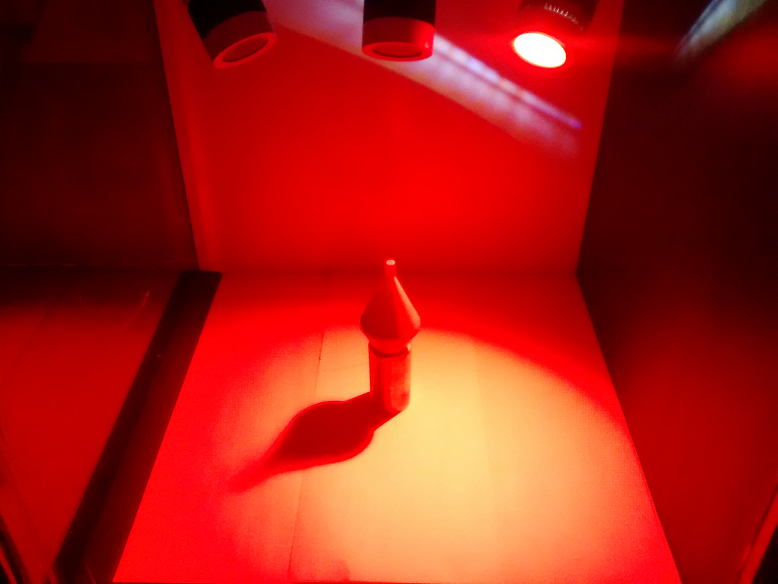
\includegraphics[width=\textwidth]{demo_1}
        \caption{A red object in red light}
        \label{img_color_demo_1}
    \end{subfigure}
    ~ %add desired spacing between images, e. g. ~, \quad, \qquad, \hfill etc. 
      %(or a blank line to force the subfigure onto a new line)
    \begin{subfigure}[b]{0.3\textwidth}
        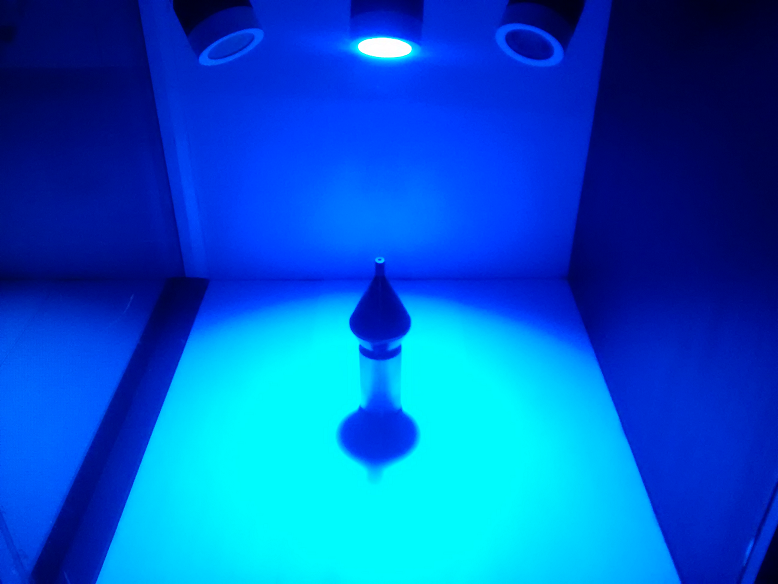
\includegraphics[width=\textwidth]{demo_2}
        \caption{A red object in blue light}
        \label{img_color_demo_2}
    \end{subfigure}
    ~ %add desired spacing between images, e. g. ~, \quad, \qquad, \hfill etc. 
    %(or a blank line to force the subfigure onto a new line)
    \begin{subfigure}[b]{0.3\textwidth}
        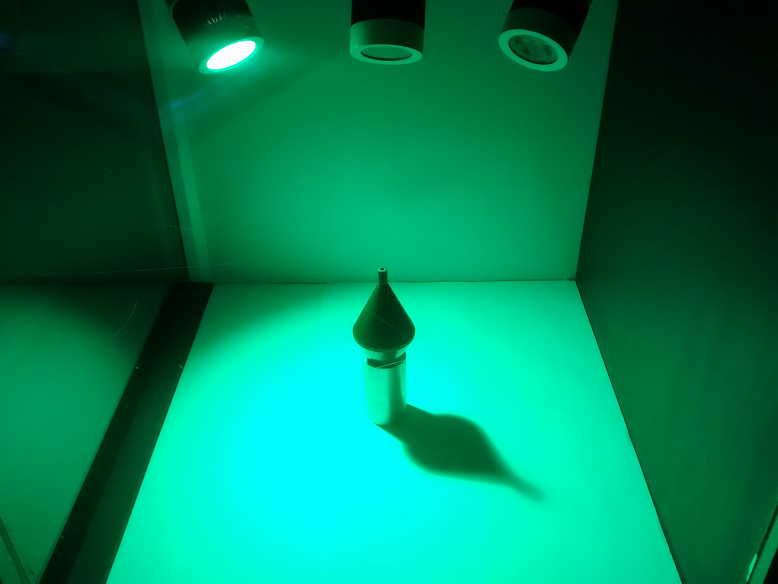
\includegraphics[width=\textwidth]{demo_3}
        \caption{A red object in green light}
        \label{img_color_demo_3}
    \end{subfigure}
    
    \begin{subfigure}[b]{0.3\textwidth}
        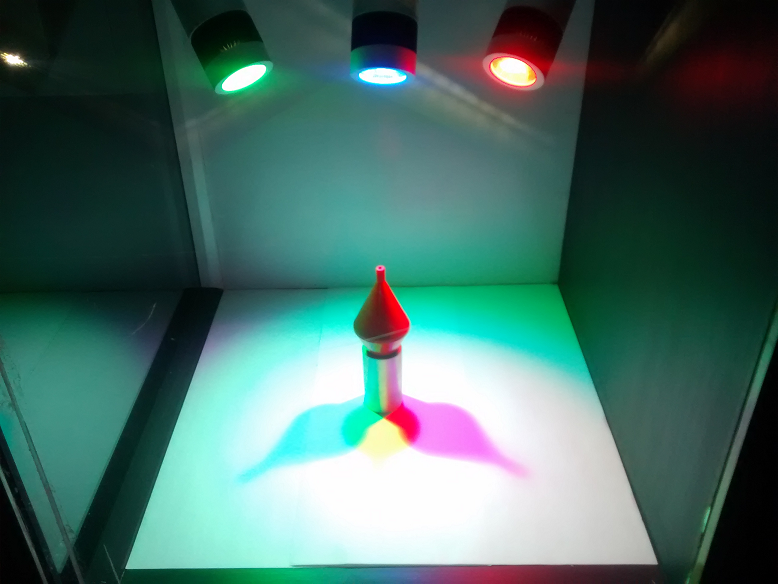
\includegraphics[width=\textwidth]{demo_4}
        \caption{The addition of colours}
        \label{img_color_demo_3}
    \end{subfigure}
    \caption{Demo on the addition of colours}\label{fig:animals}
\end{figure}

\section{The production of light}

\subsection{Thermal radiation}

Thermal radiation is the conversion of thermal energy into electromagnetic energy. But what exactly does it mean for such a transfer to occur? To understand this properly, we will of course need to understand the structure of the material that composes the matter we are providing the thermal energy to. 

Ultimately, the object producing the light is composed of constituents such as atoms and molecules arranged in some form of a lattice. You should remember from earlier courses that the \textbf{temperature} of an object is a statistical property that -- at microscopic scales -- is a reflection of the average kinetic energy of the constituents of that object. Thus, an increase in temperature would cause these atoms or molecules to start `jiggling' about more erratically (at least on an average) and would thus result in more frequent collisions between them.  

Atoms and molecules have varying behaviours when different energies are imparted to them. For example, the chemical bonds within molecules -- described by Quantum Mechanics -- vibrate at certain specific frequencies. If a collision imparts enough energy to excite one of these vibrational modes of the molecule, the kinetic energy due to the collision serves to transfer the molecule to an excited state. When it then returns back to its original state, it emits a photon having a frequency related to the energy difference between the two states. Similarly, atoms themselves have energy levels, and if a collision excites an electron to a higher level, it too returns to its ground state after emitting a photon.

The vibrational energy levels usually radiate in the infrared regime while the electronic transitions radiate in the ultraviolet. The visible region overlaps these two levels and thus obtains contributions from both. It is important to realise that since the energy is imparted through collisions, there is a continuous range of energies to which atoms and molecules may be excited and thus we get a continuous spectrum of light. However, this radiation has a very specific spectrum. It turns out that objects at the same temperature emitted more or less exactly the same spectrum of light, i.e.\ their intensities of the different wavelengths they emitted were identical. At the beginning of the last century, this was one of the `few' problems that Physics had left to address.

\subsection{Blackbody radiation and the Planck spectrum}

A black body is an idealized physical body that absorbs all incident electromagnetic radiation, regardless of frequency or angle of incidence. At thermal equilibrium (that is, at a constant temperature) it emits electromagnetic radiation called black-body radiation in the manner earlier specified. At room temperature appears it appears black, as most of the energy it radiates is infrared and cannot be perceived by the human eye. When it becomes a little hotter, it appears dull red, and as its temperature increases further it eventually becomes blue-white. The spectrum of a blackbody was known quite well experimentally, however no theoretical approach could describe the entire spectrum accurately.

At the time there were two different laws, each of which fit the experimental data in different regimes, but neither of which explained the full spectrum. For low frequencies (or long wavelengths), the law was the ``Rayleigh-Jeans law'', while for high frequencies (or short wavelengths) it was known as ``Wein's displacement law''.

\begin{figure}[!htb]
\centering
\begin{subfigure}[b]{0.45\textwidth}
        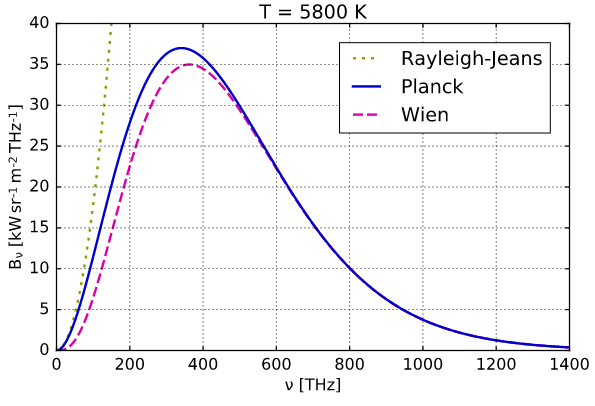
\includegraphics[width=\textwidth]{planck.png}
        \caption{Classical approximations}
        \label{planck_approx}
    \end{subfigure}
    ~ %add desired spacing between images, e. g. ~, \quad, \qquad, \hfill etc. 
      %(or a blank line to force the subfigure onto a new line)
    \begin{subfigure}[b]{0.45\textwidth}
        \hspace{0.5cm}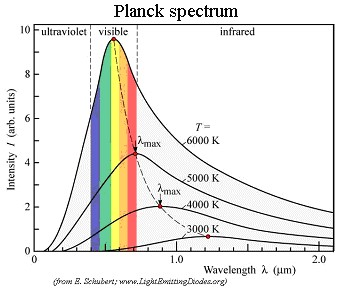
\includegraphics[width=0.8\textwidth]{planck_temp.jpg}
        \caption{Variation with temperature}
        \label{planck_temp}
    \end{subfigure}
\caption{The Planck Spectrum for Blackbodies}
\label{planck}
\end{figure}

The problem was solved by the German physicist Max Planck who realised that `classical' physics could not be used for such blackbody radiation, and thereby ushered in Quantum Mechanics by postulating that the energies were absorbed and emitted in specific quanta. The resulting spectrum was found to be characterised by the temperature of the body and was found to fit a remarkable number of spectra from the sun to the Cosmic Microwave Background Radiation left as a remnant from the Big Bang.

\begin{tcolorbox}
\paragraph{Question: } It is often said that the Cosmic Microwave Background Radiation has a `temperature' of 2.73 K. What do you think this means?
\end{tcolorbox}

\subsection{Vapour lamps and discrete spectra}

As is only to be expected, thermal radiation is not a very efficient way of producing light. The reason for this is that the radiation emitted is not restricted to only the visible spectrum and therefore much of the light that is created cannot be used to illuminate in the general sense of the word. \textbf{Vapour lamps} such as Mercury and Sodium lamps are far more efficient, essentially because they only need enough energy to excite certain electronic spectral lines of the materials within them.

In general, vapour lamps have a low pressure noble gas (Argon in the case of a Mercury lamp and a combination of Neon and Argon for Sodium). A voltage is applied to ionise the gas by creating an electrical arc: the electrons are ripped off the atoms, introducing ions, free electrons and photons into the tube. The heat from the arc vaporises the metal inside the tube. The electrons in the metal atoms then get excited to different energy levels and they cascade down to their initial states by emitting certain special frequencies (wavelengths) of light.

\begin{figure}[!htb]
\centering
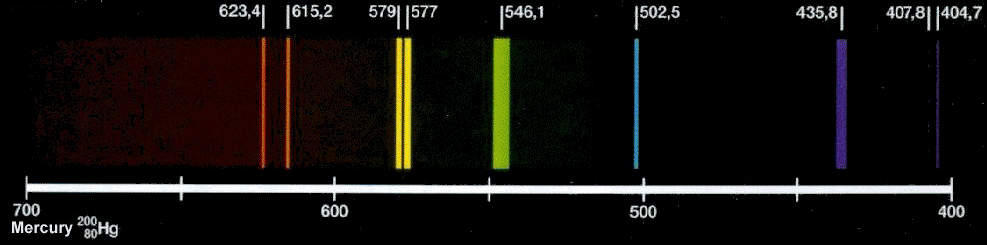
\includegraphics[width=0.75\textwidth]{hgspectrum.png}
        \caption{The mercury spectrum}
        \label{hgspectrum}
\end{figure}


\begin{tcolorbox}
\paragraph{Question: } Why do we need Quantum Mechanics to explain the spectrum you see when you look at a Mercury or Sodium vapour lamp? What would it look like if the atom were a classical object? 
\paragraph{Hint: } Consider the atom to be a `solar-system', like the Rutherford model. 

\paragraph{Question: } Can you explain the fact that you \textit{also} see a continuous spectrum on the background of the spectral lines of Sodium or Mercury when you examine their spectra?
\paragraph{Hint: } What causes a continuous spectrum?
\end{tcolorbox}

\subsection{Lasers}

Lasers are devices that emit electromagnetic radiation through a process known as \textbf{stimulated emission}. The term `Laser' itself originated as an acronym of \textit{Light Amplification by Stimulated Emission of Radiation} (which is why spelling the word with a `z' is highly incorrect). We have so far observed the production of light through a process known as \textbf{spontaneous emission} through electronic transitions within an atom. A laser differs from such sources in that it emits light \textit{coherently}, spatially and temporally. 

In the case of spontaneous emission, imagine we have two energy levels $E_0$ and $E_1$. If we manage to excite an electron in an atom to state $E_1$ , it will fall back to $E_0$ spontaneously, emitting an appropriate photon. However, both the direction and the phase of this light will be random. Furthermore, the amount of time the electron spends in this excited state (i.e.\ \textit{when} the photon is emitted) may also vary through the laws of Quantum Mechanics\footnote{Very much like the famous Heisenberg uncertainty principle $\Delta x \Delta p \geq \hbar$, there is another relation $\Delta E \Delta t \geq \hbar$ which roughly states that the time ($\Delta t$) an electron spends in state is inversely proportional to the energy difference between it and the ground state ($\Delta E$).}.

It is, however, desirable to have a coherent, monochromatic source of radiation for many different experiments (some of which you have already performed in the laboratory in these past few sessions). In order to achieve such a source, we will have to turn to another physical process known as stimulated emission.

It turns out that if we manage to excite the electron of an atom (using some sort of `pump') to the energy state $E_1$ and then \textit{pass a photon of exactly the same frequency as $\Delta E/\hbar$} near the atom, there is a very high probability that photon emitted when the $E_1 \rightarrow E_0$ transition occurs will be identical to the passing photon. In this way, we can `amplify' the original passing photon to get two photons having exactly the same phase, direction and wavelength. Such a process is known as `stimulated emission'. 

\begin{figure}[!htb]
\centering
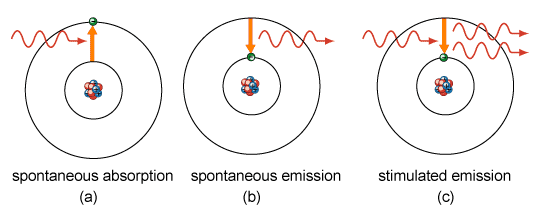
\includegraphics[scale=0.5]{img_emission.png}
\caption{Absorption, Spontaneous Emission and Stimulated Emission}
\label{img_emission}
\end{figure}

\section{The diffraction of light}

Diffraction occurs in waves when they bend around small obstacles or when they spread out after passing through narrow apertures. The standard way of analysing such a problem is some form of `Huygen's Principle', where we define \textit{wavefronts}, each point of which is the source of \textit{secondary waves} which in turn interfere, producing the pattern that you see on the screen. The introduction of these wavefronts -- albeit highly successful -- is slightly ad-hoc and not completely justified physically. This is understandable, as Huygens did not have the right tool (total integral calculus) to describe this phenomenon mathematically. Most of the mathematics was fleshed out by another great Physicist, Augustin-Jean Fresnel. This mathematics is quite involved and as I am certain that you will be subjected to it in great detail during your course on optics, I will not attempt to explain it in too much detail. 

Suffice it to say that the presence of an obstacle of a certain length $a$ in the direction of propagation of light causes some light to shift slightly and traverse a slightly larger distance. This so-called \textit{path-difference} -- dependent on the size of the obstacle $a$ -- induces a difference in \textit{phase} which in turn leads to the light interfering after it passes around the obstacle and producing a pattern of maxima and minima on the screen. Obviously, changing $a$ we would get a different pattern and so a close inspection of the interference pattern provides us with information on the dimension of the obstacle.

\subsection{Babinet's Principle}

Babinet's principle states that

\begin{center}
\textit{Complementary objects produce the same different pattern, except for the intensity of the central maxima.}
\end{center}

We will provide a quick `proof' of this after some mathematical baggage in the subsequent sections. 

\begin{tcolorbox}
\paragraph{Question: }Two objects are complementary if one of them is transparent when the other is opaque and opaque when the other is transparent. What are the complementary objects of the following:

\begin{enumerate}
\item A narrow slit of width $d$.
\item A circular aperture of diameter $d$.
\end{enumerate}
\end{tcolorbox}

Henceforth we will not differentiate between the patterns made by such complementary objects.

\subsection{The single slit}

When the path difference due to a single slit (or thin wire) is exactly equal to an integral number of wavelengths of the light used, the waves \textit{interfere destructively}. As a result, minima occur whenever

\begin{equation*}
\underbrace{a \sin{\theta_n}}_{\text{path difference}} = \underbrace{n \lambda}_{\substack{\text{integral number} \\ \text{of wavelengths}}}
\end{equation*}

I would like to stress that the above way of interpreting mathematical equations is very important, as it attaches a physical significance to every mathematical entity in the equation.


\begin{tcolorbox}
\paragraph{Question: } What happens to $\theta_n$ when you increase $a$? 

\paragraph{Question: } Using the above equation, what is the \textbf{smallest} length you can probe using a light of wavelength $\lambda$? Prove this mathematically.

\paragraph{Question: } Is there a maximum length above which light of a wavelength $\lambda$ can no longer probe? If yes, prove it mathematically. If no, what additional constraints are introduced when probing larger length scales?
\end{tcolorbox}

Observing the pattern in Figure \ref{img_diff} you can clearly see that the intensity is not a constant, but seems to vary with angle. It turns out that -- as a function of the angle $\theta$ -- the intensity falls as 

\begin{equation*}
I(\theta) = I(0) \left( \frac{\sin{\beta}}{\beta}\right)^2 \quad \quad \text{where  } \beta = \frac{\pi a \sin \theta}{\lambda}
\end{equation*}

\begin{figure}[!htb]
\centering
    \begin{subfigure}[b]{0.45\textwidth}
        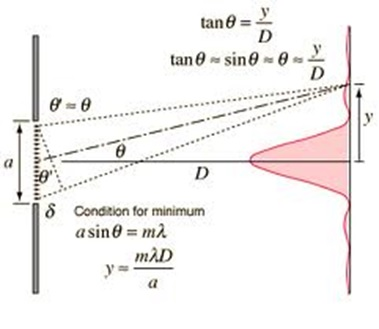
\includegraphics[width=0.8\textwidth]{fraun_theory.jpg}
     %   \caption{}
        \label{fraun_theory}
    \end{subfigure}
\begin{subfigure}[b]{0.45\textwidth}
       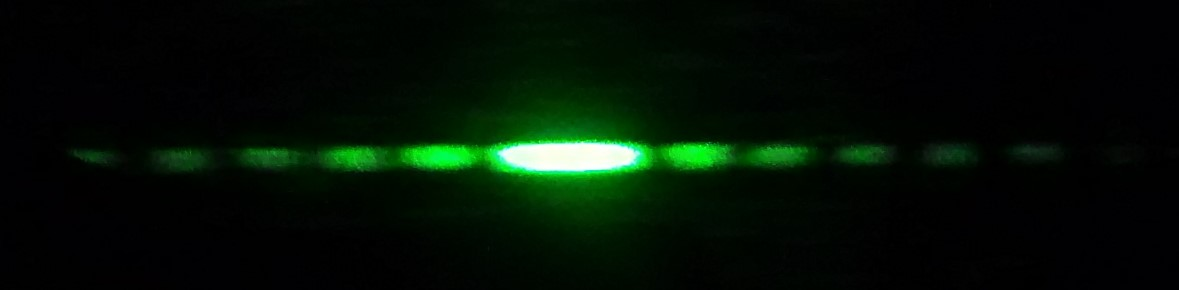
\includegraphics[scale=0.2]{fraun.jpg}
     %   \caption{Pattern on the screen}
        \label{fraun}
    \end{subfigure}
\caption{Diffraction pattern due to a single slit}
\label{img_diff}
\end{figure}


\begin{tcolorbox}
\paragraph{Question: } Can you sketch the above function? Write down an equation to find its zeros. Does it look familiar?
\end{tcolorbox}

\subsection{The single helix}

The single helix has, associated with it, two length scales: the thickness of the wire and the spacing between the wires (the `pitch'). The pitch works wither as two thin wires separated by a distance $P$, or alternatively a single slit of width $P$.

The entire pattern can thus be decomposed into a diffraction grating angled up at an angle $\alpha_1$, a diffraction grating angled down at an angle $\alpha_1$ (both of which have a thickness $a$), and diffraction gratings angled up (and down) at the same angle (of thickness $P$). Thus, these four objects combine together to get the $X$ shaped pattern on the screen.

\subsection{The double helix}

This pattern can be decomposed in a very similar fashion as the single helix, except that there is now another length scale associated with the object: the \textit{separation} between the two helices $d$, which produces another diffraction pattern on each arm of the $X$.



\begin{figure}[!htb]
\centering
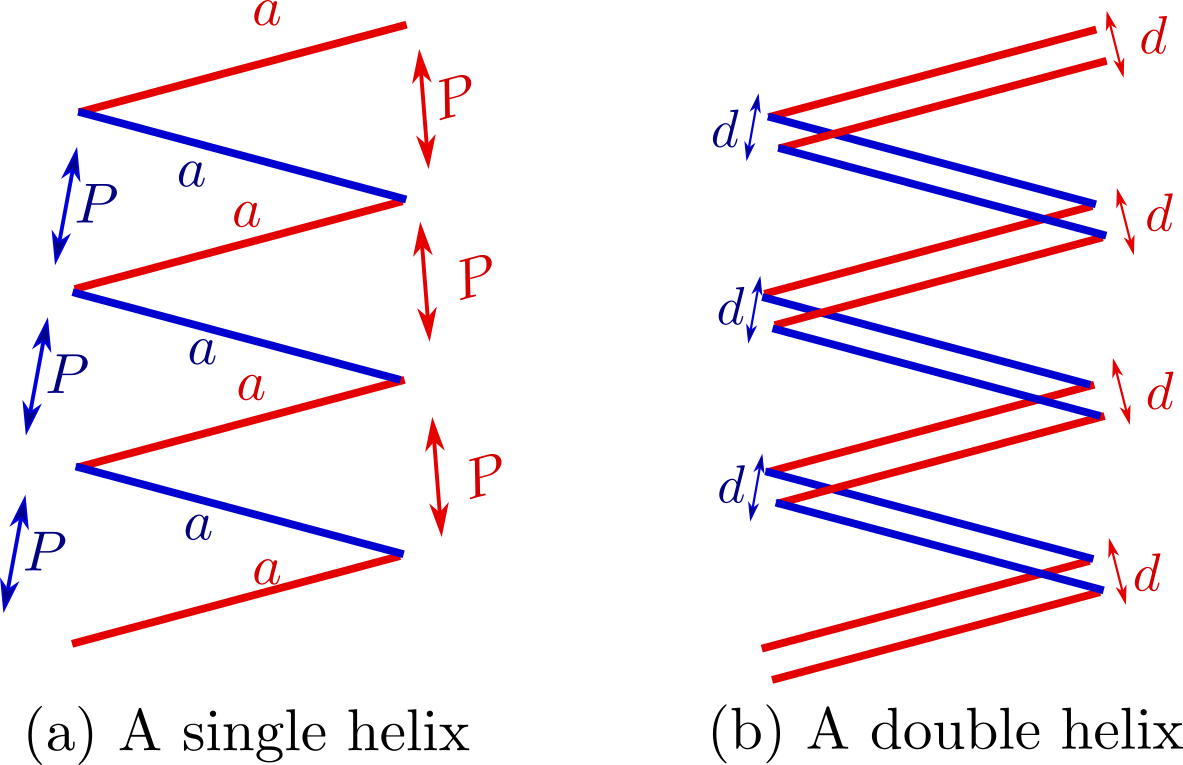
\includegraphics[scale=0.2]{helices.png}
\caption{Schematics of a single and double helix}
\label{helix}
\end{figure}



\section{The Fourier Transform}

It turns out that the diffraction patterns and the obstacles that produce them are very closely related by an extremely cool mathematical relationship called a \textbf{Fourier Transform}. You will be studying about this in great detail in your mathematical physics courses and -- should you wish to continue in Physics --  it will be impossible for you to avoid it in the future. The Fourier Transform, as you might imagine, is quite closely related in principle to the Fourier Series you have already encountered and I will try to motivate this relationship in the subsequent sections.

\subsection{The epicycles}

As I was researching for this class I discovered something absolutely fabulous that I thought I \textit{had} to tell you. To understand this, we will have to go back to the oldest natural science: astronomy. The Greeks -- as most cultures of antiquity -- were very interested in the motions of the heavens. They were also very interested in symmetry and harmony, different ideas which found a synthesis in many of their theories of the world. 

The sphere, of course, being extremely symmetric was their orbit of choice to describe the heavens. Plato (circa 400 BC) came up with the notion of the Earth at the center of the universe and all other objects orbiting it in spherical trajectories. There were, however, certain annoying heavenly bodies that refused to behave as expected. These were called `wanderers', \textit{planétai}. The motion of these planets caused them considerable distress, as they were quite a fly in the ointment of symmetry. A solution to the problem was provided by Ptolemy.

The problem was that if you watch the planets carefully, they sometimes move backwards in the sky. So Ptolemy came up with the following idea: planets move around one big circle, but they move around a little circle at the same time. Imagine spinning a stick around you, the edge of which is attached to a rotating wheel. The planet would move like a point on the edge of the wheel; these circles were known as `epicycles'. This theory turns out to be wrong, but more importantly it is a \textit{bad} theory, for a reason that we shall soon see. It turns out that the orbit of any planet -- viewed from earth -- can be described to arbitrary accuracy by adding enough epicycles, as can be seen \href{https://www.youtube.com/watch?v=QVuU2YCwHjw}{in this amazing YouTube video}.

\begin{figure}[!htb]
\centering
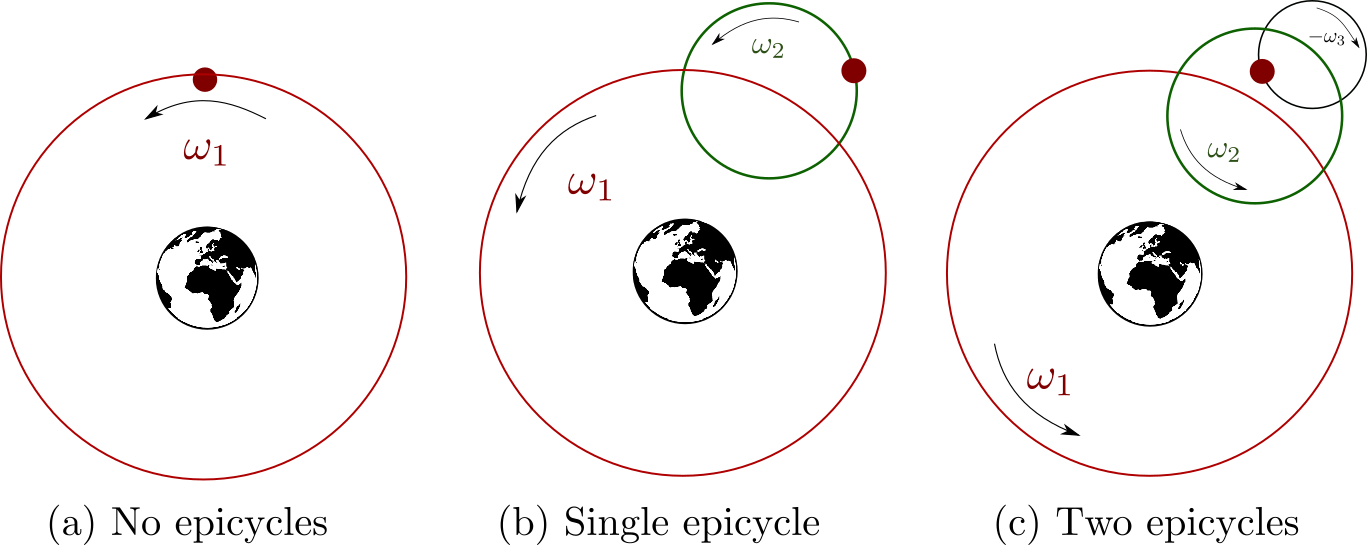
\includegraphics[scale=0.4]{epicycles.png}
\caption{Epicycles and planetary motion}
\label{epicycles}
\end{figure}

The planet moves about in trajectory on a plane. Let us try to understand this mathematically. An easy way to do this in two dimensions is to superimpose a complex plane over real space and consider the motion of this particle as if it were moving about in this plane. You can easily justify this to yourself realising that circles are much easier to represent using complex numbers. The motion of a point on the edge of a single circle rotating at a frequency $\omega$ and having a radius $R$ is given by

\begin{equation*}
z(t) = R e^{i \omega t}
\end{equation*}

For two circles it would be 


\begin{equation*}
z(t) = R_1 e^{i \omega_1 t} + R_2 e^{i \omega_2 t}
\end{equation*}

We could now imagine adding three, four, or even an infinite number of circles, with every possible angular frequency. In this case, the sum would become an \textit{integral}, and the discrete indices of $R_1, R_2, ...$ etc. will be replaced by a continuous function $R(\omega)$. Thus,


\begin{equation*}
z(t) = \int^\infty_{-\infty} R(\omega) e^{i \omega t} \dd \omega
\end{equation*}

This new function $R(\omega)$ is called the Fourier Transform of $z(t)$. Giving you the function $R(\omega)$ is equivalent to giving you all the information in $z(t)$.

Let's examine what this means. It means that any arbitrary time dependent function $z(t)$ can be perfectly emulated by infinitely many circles of different frequencies all added up, provided that their radii are `correctly' weighted with respect to their frequencies (the function $R(\omega)$ we just saw). We could now add a further constraint that would simplify our analysis. Suppose now that the function is \textbf{periodic}, meaning that the path closes back on itself. Then, most frequencies  are no longer necessary, and only integral values of the frequency of the slowest circle contribute to the function. In this case, the integral reverts back to an infinite countable sum.


\begin{equation*}
z(t) = \sum_{n = -\infty}^\infty R_n e^{i n \omega_0 t}
\end{equation*}

which should look familiar. You could that the first ten or twenty and ignore the rest, fitting the data to any level of precision you wish.

\subsection{The inverse transform}

Diffraction, as I already mentioned, produces a pattern on the screen that is a Fourier Transform of the obstacle or aperture.We will use this face to ``prove'' Babinet's Principle, however we still have a little more math to get out of the way. 

We have already seen that if we use the earlier mentioned formula for the Fourier Transform\footnote{The actual definition of the Fourier Transform and its inverse are occasionally reversed, and there are also factors of $2\pi$ that appear and disappear. These, however, do not affect our strictly qualitative analysis.}, then you can also invert the operation exactly as you would in the case of Fourier series. 

\begin{tcolorbox}

\paragraph{Forward Fourier Transform}

\begin{equation*}
z(t) = \int^\infty_{-\infty} R(\omega) e^{i \omega t} \dd \omega
\end{equation*}

\paragraph{Inverse Fourier Transform}

\begin{equation*}
R(\omega) = \int^\infty_{-\infty} z(t) e^{-i \omega t} \dd t
\end{equation*}

\paragraph{Note: } Notice that the two variables $t$ and $\omega$ in question here are related inversely. This is characteristic of Fourier Transforms.

\end{tcolorbox}

\subsection{The Dirac Delta function}

The last mathematical object that we will have to deal with is the Dirac Delta function that most of you must have already heard of. It is a strange function\footnote{Later, you will learn that it is not really even a function, but rather a \textit{distribution}.}. This function is zero everywhere, except at the origin where it is infinite.

\begin{equation*}
\delta (k) = \begin{cases}
              \infty, & k = 0\\
               0,              & \text{otherwise}
             \end{cases}
\end{equation*}

It is defined by its action on other functions. In particular,

\begin{equation*}
\int_{-\infty}^\infty \delta(k) f(k) \dd k = f(0)
\end{equation*}

i.e.\ it picks up \textit{only} the value at 0.

\begin{tcolorbox}
\paragraph{Question: } What is the Fourier Transform of $\delta(k)$?

\paragraph{Question: } What do you think is the Fourier Transform of 1?
\paragraph{Answer: } It turns out to be $\delta(k)$.
\end{tcolorbox}


\subsection{Proving Babinet's Principle}

Here is a rudimentary proof of Babinet's principle. Let us begin by drawing out two complementary objects, a slit and a thin wire of the same thickness.

\begin{figure}[!htb]
\centering
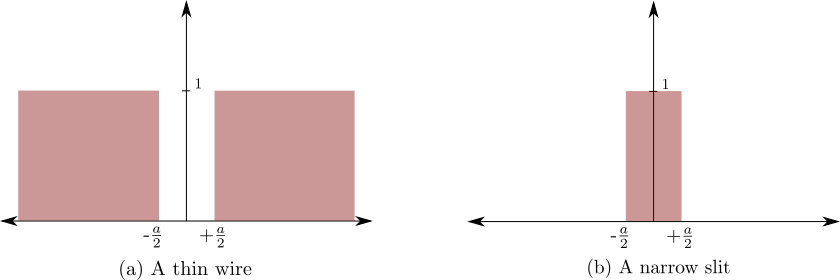
\includegraphics[scale=0.5]{complementary.png}
\caption{Complementary objects: A thin wire and a narrow slit}
\label{img_complementary}
\end{figure}

Let us suppose that we add both of these objects. The resulting pattern will simply be 1, as they are complementary. This will happen to any pair of complementary objects. Thus,

\begin{equation*}
f(x) + f_\text{comp}(x) = 1
\end{equation*}

We know the following three things:

\begin{enumerate}
\item The Fourier Transform is linear (since its an integral),
\item The Fourier Transform represents what we will see on the screen.
\item The Fourier Transform of 1 is $\delta(k)$.
\end{enumerate}

Thus, if we call $\widetilde{f}(k)$ and $\widetilde{f}_\text{comp}(k)$ the Fourier transforms of $f(x)$ and $f_\text{comp}(x)$, then taking the Fourier transforms of the last equation, we get

\begin{equation*}
\widetilde{f}(k) + \widetilde{f}_\text{comp}(k) = \delta(k)
\end{equation*}

Now this might appear to be a particularly formidable equation to solve, but we shall solve it \textit{à la physicienne}. The Dirac Delta is zero almost everywhere. In fact, it is zero everywhere \textit{except} at the origin (i.e.\ everywhere that Babinet's principle holds!) and so we shall consider every point \textit{except} the point directly in front of the beam\footnote{Remember that Babinet's principle also does not hold for the intensity of the central beam.}. Of course, in this case, $\delta(k) = 0$. Thus,

\begin{equation*}
\widetilde{f}(k) + \widetilde{f}_\text{comp}(k) = 0
\end{equation*}

or in other words,

\begin{equation*}
\widetilde{f}(k) = - \widetilde{f}_\text{comp}(k)
\end{equation*}

which, you will appreciate, is simply a mathematical formulation of Babinet's principle.

\subsection{Examples}

Here are some quick examples, convince yourselves that the mathematical description of the apertures is accurate. The function $\Theta(x)$ is known as Heaviside Step Function. It is defined as

\begin{equation*}
\Theta (x) = \begin{cases}
              0, & x < 0\\
              1, & x > 0
             \end{cases}
\end{equation*}


\begin{figure}[!htb]
\centering
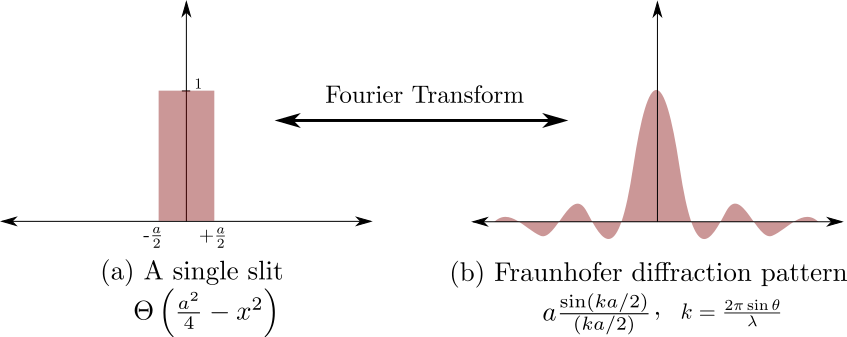
\includegraphics[scale=0.4]{example_1.png}
\caption{A single slit}
\label{example_1}
\end{figure}

\begin{figure}[!htb]
\centering
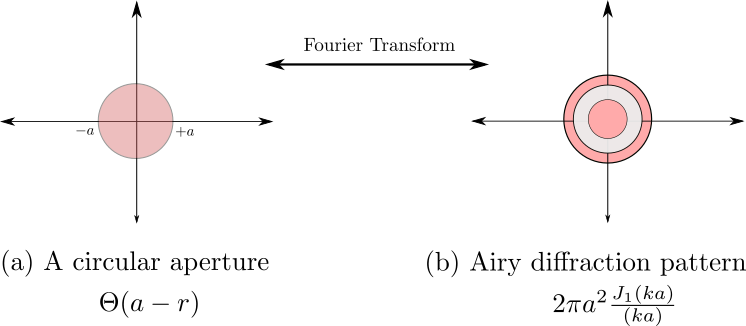
\includegraphics[scale=0.4]{example_2.png}
\caption{A circular aperture}
\label{example_2}
\end{figure}


\begin{tcolorbox}
\paragraph{Remark: } $J_1(ka)$ is a special function known as a \textbf{Bessel function}. It occurs very frequently in Physics. You may think of it as a ``modified'' sine function, except that instead of at $x=n\pi$, the function has zeros at different values, specified on Figure \ref{example_3} below.

\paragraph{Question: } Can you explain the fact that for circular apertures, the values of $\bar{m}$ are not integers. Can you explain their values?
\end{tcolorbox}

\begin{figure}[!htb]
\centering
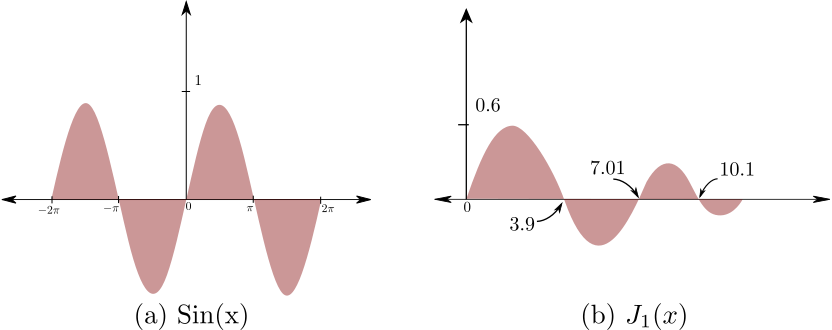
\includegraphics[scale=0.4]{example_3.png}
\caption{The Bessel function as a modified sinusoid}
\label{example_3}
\end{figure}

\newpage

\section*{References and additional reading}

\begin{enumerate}
\item \href{https://physics.info/planck/}{Blackbody Radiation - The Physics Hypertextbook}
\item \href{https://www.ifa.hawaii.edu/~barnes/ASTR110L_F05/spectralab.html}{Spectra in the Lab}
\item \href{http://hyperphysics.phy-astr.gsu.edu/hbase/quantum/atspect.html}{Atomic Spectra - Hyperphysics}
\item \href{https://pdfs.semanticscholar.org/8ccd/de212e9059a35c111704073aea2443984614.pdf}{How Rosalind Franklin Discovered the Helical Structure of DNA: Experiments in Diffraction}
\item \href{https://physics.stackexchange.com/questions/383138/diffraction-pattern-due-to-double-helix?rq=1}{Diffraction of a double helix - Physics StackExchange}
\item \href{https://betterexplained.com/articles/an-interactive-guide-to-the-fourier-transform/}{An Interactive Guide To The Fourier Transform}
\item \href{https://nipunbatra.github.io/blog/2016/FT.html}{Dummies guide to Fourier Transform} (This involves programming using Python)
\item \href{https://math.stackexchange.com/questions/1002/fourier-transform-for-dummies}{Fourier Transform for Dummies - Mathematics StackExchange}
\item \href{https://www.youtube.com/watch?v=QVuU2YCwHjw}{Ptolemy and Homer (Simpson) - YouTube}
\item \href{http://brettcvz.github.io/epicycles/}{The Epicycle Demonstrator - Drawing by Epicycles} (This site has some wacky examples, including the letter 'B')
\item \href{http://www.cchem.berkeley.edu/chem120a/extra/delta_functions.pdf}{Delta Functions}
\end{enumerate}


\clearpage
\pagenumbering{arabic}

\part{Assessment}

\title{\vspace{-2cm} PHY102: Conceptual and Procedural Understanding\\\vspace{0.25cm} {Written examination}}
\author{}
\date{\vspace{-2cm} 4th May, 2018}

\maketitle
\vspace{-1.5cm}
\begin{center}
\hrulefill\\
\textbf{Instructions:}

\begin{itemize}
\item \textbf{Read the question paper carefully!}
\item The total duration of the written exam is \textbf{90 minutes}.
\item You are required to return the question paper with your answer sheet.
\item \textbf{No} electronic devices of any kind will be allowed during the examination.
\item Multiple choice questions and sketches must be marked on the question paper \textbf{clearly}.
\end{itemize}
\vspace{-0.9cm}
\hrulefill
\end{center}
\vspace{-0.9cm}
\section*{Multiple Choice Questions \hfill (5 marks)}

\begin{enumerate}
\item What is the distance between two successive divisions on the Vernier scale of a Vernier caliper of least count 0.02 mm?
\begin{enumerate}
\item 1 mm
\item 1/50 mm
\item 49/50 mm \hfill \textbf{(1 mark)}
\end{enumerate}


% \item With water, the colour red of a rainbow is observed at $42^\circ$. Supposing instead you had an acid solution (of density 1.5 g/cc). Red will now appear at:
% \begin{enumerate}
% \item An angle greater than $42^\circ$,
% \item An angle less than $42^\circ$,
% \item The same angle.\hfill \textbf{(1 mark)}
% \end{enumerate}


\item Why was a lens used in the Formation of Rainbow experiment? \hfill \textbf{(1 mark)}

\begin{enumerate}
\item To concentrate the light from the bulb onto the drop.
\item To make the light rays from the source parallel.
\item To create a point source from an extended source.
\end{enumerate}

\item You are given three laser sources which emit light of wavelengths $\lambda_1$, $\lambda_2$ and $\lambda_3$. On passing them through a fixed grating -- keeping all else constant -- the pattern of bright spots on the screen is observed as shown in Figure \ref{lambdaGratings}. Which of the following is true? \hfill \textbf{(2 marks)}

\renewcommand{\figurename}{\hspace{4cm} Figure}


\begin{figure}[!htb]\hspace{2cm}
\centering
\hspace{2cm}
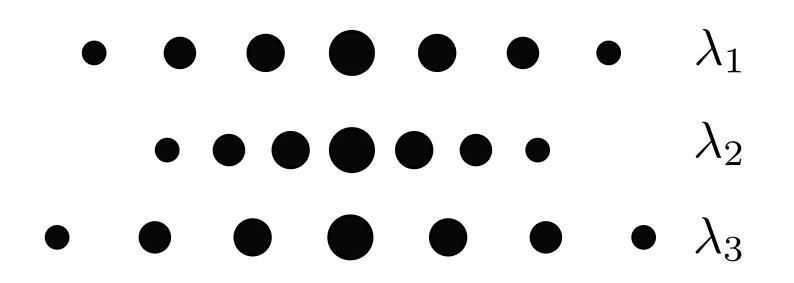
\includegraphics[width=0.5\textwidth]{q10.png}%
\hfill\caption{How are the $\lambda$s related?}
\label{lambdaGratings}
\end{figure}
\vspace{-4cm}
\begin{enumerate}
\item $\lambda_1 > \lambda_2 > \lambda_3$
\item $\lambda_1 < \lambda_2 < \lambda_3$
\item $\lambda_2 < \lambda_1 < \lambda_3$
\item $\lambda_2 > \lambda_1 > \lambda_3$
\item $\lambda_2 > \lambda_3 > \lambda_1$
\end{enumerate}
\vspace{0.5cm}


\renewcommand{\figurename}{Figure}
\newpage
\item Three identical $12$ V bulbs (rated at 21W) are arranged in a circuit as indicated in Figure \ref{bulbGlow}. Which of the following is/are true? \hfill \textbf{(1 mark)}


\renewcommand{\figurename}{\hspace{5cm} Figure}
\vspace{-0.5cm}
\begin{figure}[!htb]
\hspace{4cm}
\centering
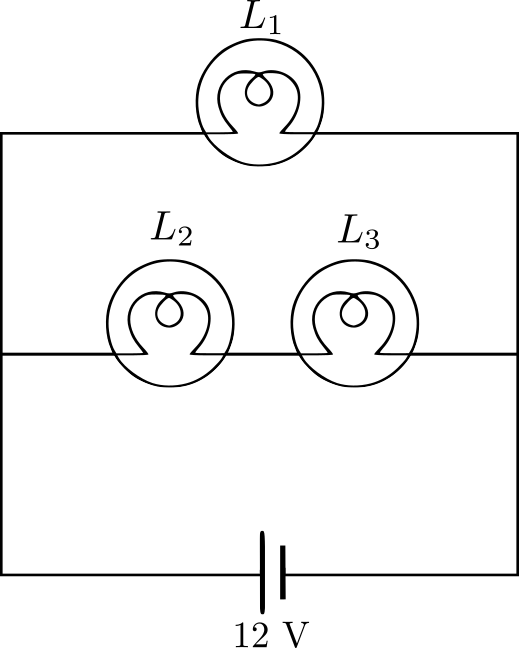
\includegraphics[width=0.25\textwidth]{q1.png}
\caption{}
\label{bulbGlow}
\end{figure}

\vspace{-5cm}

\begin{enumerate}
\item $L_1$ glows the brightest,
\item $L_2$ and $L_3$ glow equally brightly,
\item $L_2$ glows brighter than $L_3$,
\item $L_1$ and $L_2$ glow equally brightly.
\end{enumerate}

\vspace{2.5cm}
\renewcommand{\figurename}{Figure}

\section*{Short Answer Questions \hfill (10 marks)}



% \item State Babinet's principle and explain it with the help of an example, describing in detail the diffraction patterns observed.  \hfill \textbf{(1 mark)}


% \item What are the smallest and largest lengths that can be theoretically measured by diffraction using light of a wavelength 532 nm. Justify your answer. \hfill \textbf{(2 marks)}



\item Why does the intensity of light of a point source fall off as the inverse square of the distance from the source? \hfill \textbf{(2 marks)}


\item If $f'_0$ is the fundamental frequency of a massive spring with one end clamped, and $f_0$ is the fundamental frequency of the same spring with both ends clamped, explain why $f_0 = 2 f'_0$. You may use a suitable analogy if required. \hfill \textbf{(2 marks)}

% \item A single slit of width $a$ is placed in the way of a laser. The normalised intensity of the diffraction pattern is plotted against a function ($\pi a \sin\theta / \lambda$) of the angular separation $\theta$ as shown in Figure \ref{intensityPattern}. On the same figure (Figure \ref{intensityPattern}), sketch the pattern if the slit width is doubled. \hfill \textbf{(1 mark)}

% \begin{figure}[!htb]
% \centering
% 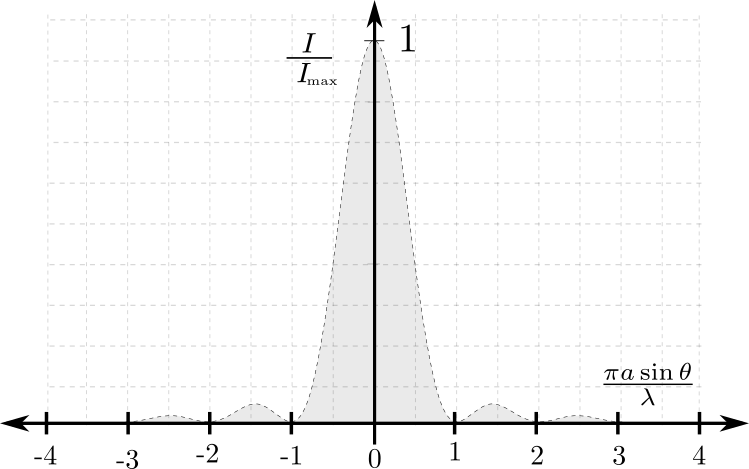
\includegraphics[width=0.85\textwidth]{q8.png}
% \caption{Sketch the new pattern on the graph.}
% \label{intensityPattern}
% \end{figure}


\item Suggest a method to increase the intensity of the light falling on the drop in the Formation of Rainbow experiment, assuming that we cannot change the bulb or power supply. You have at your disposal many lenses of different sizes, focal lengths and powers. \hfill \textbf{(2 marks)}

\item Sketch the following graphs for a simple pendulum that is left from rest at a small angle $A$.

\begin{enumerate}
\item Position vs. Time
\item Velocity vs. Time 
\item Acceleration vs. Time \hfill \textbf{(2 marks)}
\end{enumerate} 

\item Roughly sketch a graph of the \textit{residence time} of the above-mentioned pendulum over a single cycle in Figure \ref{resGraph}. The residence time is defined as the amount of time ($\Delta t$) that the pendulum spends in a region of space ($\Delta x$). \hfill \textbf{(2 marks)}

\begin{figure}[!htb]
\centering
\begin{subfigure}[b]{0.5\textwidth}
\centering
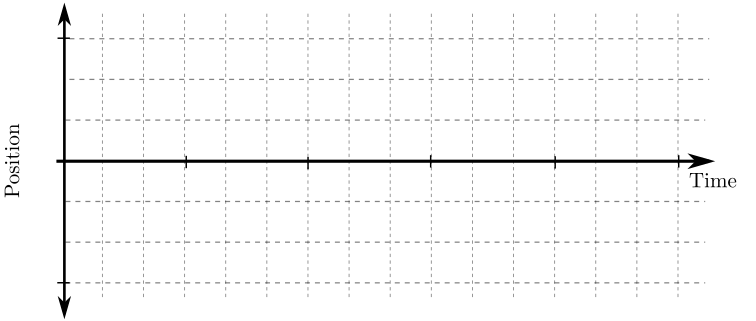
\includegraphics[width=\textwidth]{q11.png}
\caption{Question 9(a)}
\end{subfigure}%
\begin{subfigure}[b]{0.5\textwidth}
\centering
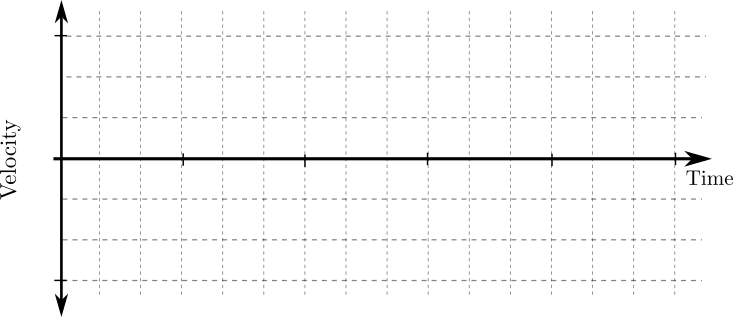
\includegraphics[width=\textwidth]{q12.png}
\caption{Question 9(b)}
\end{subfigure}
\begin{subfigure}[b]{0.5\textwidth}
\centering
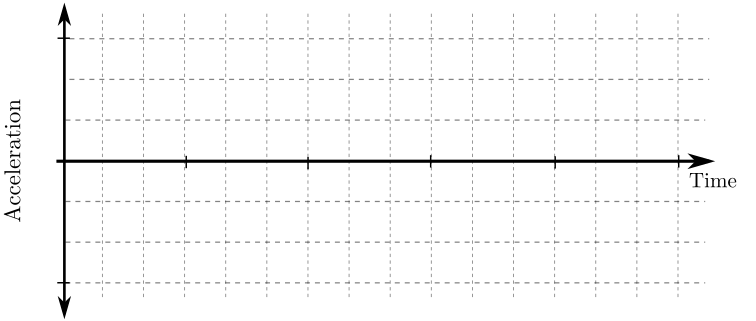
\includegraphics[width=\textwidth]{q13.png}
\caption{Question 9(c)}
\end{subfigure}
\end{figure}



\begin{figure}[!htb]
\centering
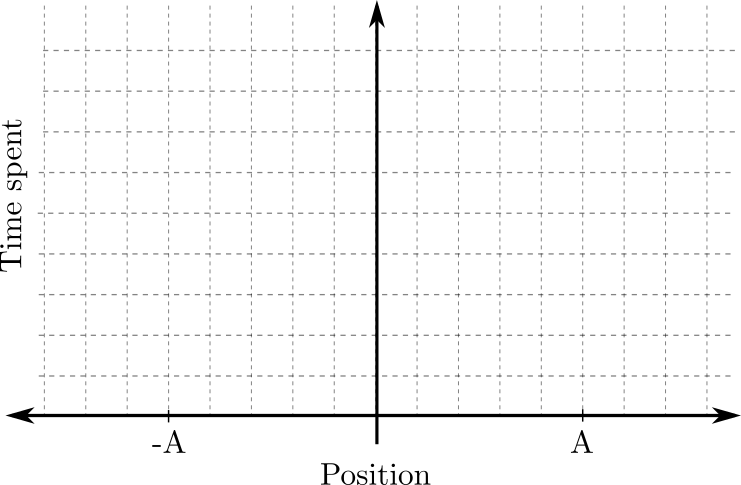
\includegraphics[width=0.85\textwidth]{q7.png}
\caption{Sketch a graph of residence time versus position.}
\label{resGraph}
\end{figure}

\newpage
~\\
~\\
\newpage
\section*{Long Answer Questions \hfill (15 marks)}



\item You are conducting an experiment to measure the time period of a simple pendulum using a \textbf{stopwatch}. At which point of the trajectory would you start counting the number of cycles? 

Now suppose instead that you are using a \textbf{digital sensor} to detect the pendulum's position. At which point of the pendulum's trajectory would you place such a sensor if you want to count the number of cycles?

Justify your answer in both the above cases. (\textbf{Hint:} You can use your answer from Question (9).)  \hfill \textbf{(3 marks)}


\item Why was soap solution used in the Surface Tension experiment? How much soap should one ideally use for the experiment? Justify your answer. \hfill \textbf{(3 marks)}



\item In the experiment for the Characterisation of an Incandescent Lamp, the circuit is set up as shown in Figure \ref{incandCirc} with a 12V lamp rated at 21W. However, the bulb is found to not glow. Explain why this happens.  \hfill \textbf{(3 marks)}

\begin{figure}[!htb]
\centering
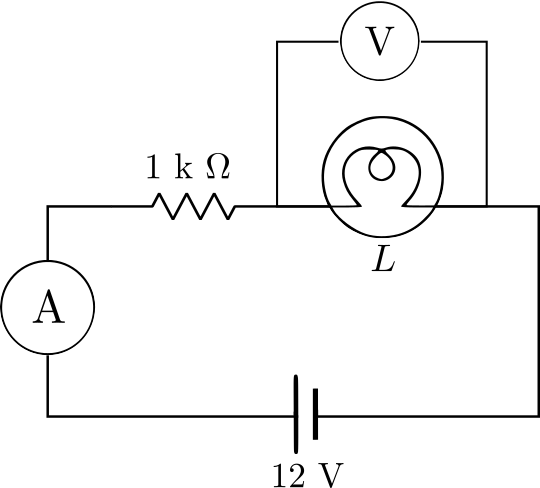
\includegraphics[width=0.25\textwidth]{q2.png}
\caption{Explain why the bulb does not glow.}
\label{incandCirc}
\end{figure}


\item Design an experiment to find the resistance of a fuse (rated 500 mA). You are provided with a power supply ($0-5$V), two digital multimeters, and a resistance ladder. Make sure you mention \textbf{all} necessary details, including the settings of the multimeter, and provide a circuit diagram. \hfill \textbf{(3 marks)}



% \item The displacement of the free end of a slinky spring clamped at its upper end and oscillating vertically is given by 

% \begin{equation*}
% Y = A e^{-\left(\frac{b}{2m}\right) t}\cos{\omega t}
% \end{equation*}

% \noindent where $A$, $b$, $\omega$ and $m$ are constants and $t$ is time. Design an experiment to determine the factor $b/m$. Mention all the stages of data collection and interpretation, including the number of readings you will take and why, as well as graphs you will plot (if any). \hfill \textbf{(5 marks)}


% \item When drops are formed on a plane surface due to Surface Tension, the following relations are found to hold true:

% \begin{equation*}
% \begin{aligned}
% T &= k \cdot m \cdot g\\
% T &= C \cdot r^x \cdot d^y
% \end{aligned}
% \end{equation*}

% \noindent where $k$ and $C$ are constants, $r$ is the radius of the formed drop and $d$ the density of the solution. $x$ and $y$ are numbers. Design an experiment to find $x$. You are provided with a \textbf{glass plate}, \textbf{soap powder}, a \textbf{weighing balance} and \textbf{beakers}. You may include other objects if required.  \hfill \textbf{(3 marks)}



% \item Describe the diffraction pattern you would obtain using a Double Helix, indicating clearly which parameter of the Double Helix governs which parameter in the pattern. \hfill \textbf{(3 marks)}



\item Sketch the IV Characteristics of the circuits represented in Figure \ref{IVChar}. State the units on the axes of the graphs, as well as the rough values of voltage and current which characterise the circuit. \hfill \textbf{(3 marks)}

\begin{figure}[!htb]
\centering \hfill
\begin{subfigure}[b]{0.5\textwidth}
\centering
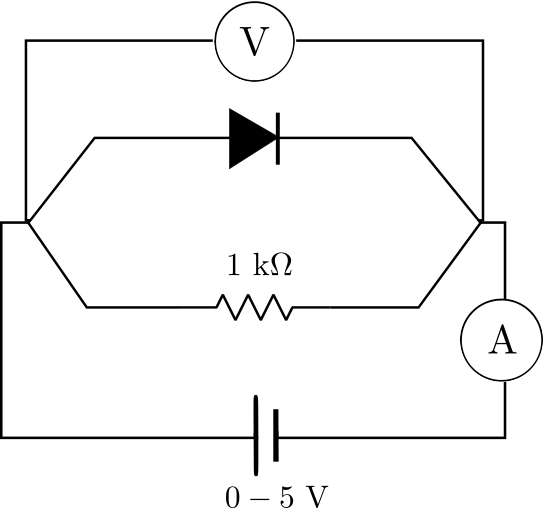
\includegraphics[width = 0.5\textwidth]{q3.png}
\end{subfigure}\hfill
\begin{subfigure}[b]{0.5\textwidth}
\centering
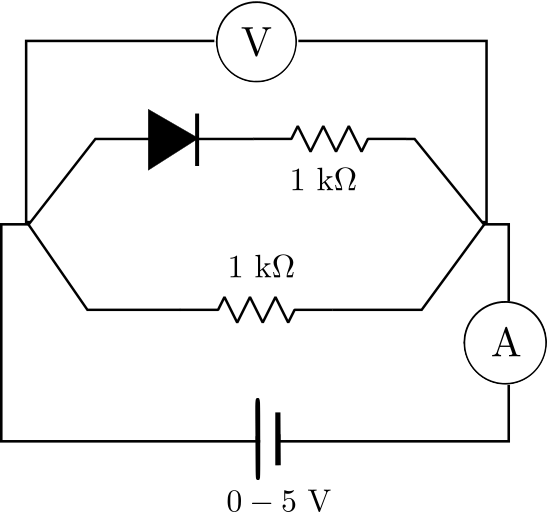
\includegraphics[width = 0.5\textwidth]{q4.png}
\end{subfigure}%
\hfill
\caption{Question 14 | Sketch the IV Characteristics}
\label{IVChar}
\end{figure}



% \begin{figure}[!htb]
% \centering
% 
\includegraphics[width=0.85\textwidth]{q9.png}
% \vspace{1.5cm}
% \caption{Sketch the pattern for a thin wire of thickness 1 mm.}
% \label{diffractionSlit}
% \end{figure}
\end{enumerate}

\begin{figure}[!htb]
\centering
\begin{subfigure}[b]{\textwidth}
\centering
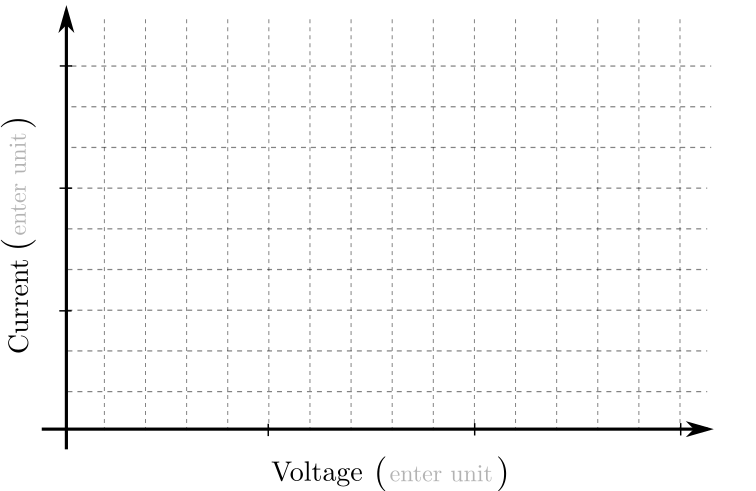
\includegraphics[width=\textwidth]{q6.png}
\caption{Question 14(a)}
\end{subfigure}
\begin{subfigure}[b]{\textwidth}
\centering
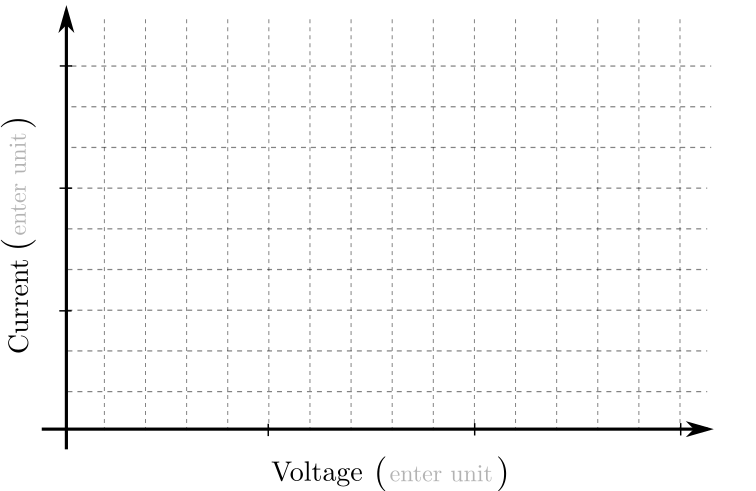
\includegraphics[width=\textwidth]{q6.png}
\caption{Question 14(b)}
\end{subfigure}
\end{figure}

\clearpage
\pagenumbering{arabic} 

\end{document}